\chapter{Desarrollo}

\section{Estudio del modelo matemático del PMSM}

En esta sección, se abordará de manera gradual la introducción al control vectorial de máquinas eléctricas. Esta sección se asemeja más a un conjunto de pasos para comprender completamente el control utilizado en los inversores. Es importante tener en cuenta que existen muchas simplificaciones matemáticas, suposiciones no justificadas y pasos omitidos ya que la extensión de la sección sería extremadamente larga en caso de razonar desde cero todos los resultados.

\subsection{Modelo trifásico del PMSM}

Los motores síncronos de imanes permanentes (PMSM) están hechos de hierro, cobre y imanes. Se limita el análisis a máquinas de tres fases, aunque el análisis para sistemas con más de tres fases es similar. El cobre se distribuye en devanados, que tienen una resistencia y una inductancia iguales entre ellas si la máquina está equilibrada. Además, cuando el rotor gira, los imanes permanentes inducen una tensión en los devanados, lo que se conoce como fuerza contra-electromotriz (FCEM).

Se trabajará con motores cuyos devanados estén conectados en configuración estrella, ya que se utiliza con mucha más frecuencia que la configuración delta. Por lo tanto, se puede construir un circuito eléctrico equivalente simple. De todas maneras, es sencillo extender el modelo y el control a motores con conexión estrella.


\begin{figure}[!ht]
	\centering
	\begin{circuitikz}
		% Draw three phases
		\draw (0,0) to [L, l=$L_s$, o-] ++(2,0) to [R, l=$R_s$] ++(2,0) to [sV, v=$e_a$, invert] ++(2,0) -- ++(0,-2){};
		
		\draw (0,-2) to [L, l=$L_s$, o-] ++(2,0) to [R, l=$R_s$] ++(2,0) to [sV, v=$e_b$, invert] ++(2,0) -- ++(0,2);
		
		\draw (0,-4) to [L, l=$L_s$, o-] ++(2,0) to [R, l=$R_s$] ++(2,0) to [sV, v=$e_c$, invert] ++(2,0) -- ++(0,2);
		
		% Draw neutral point
		\draw (6,-2) node[circ]{} -- ++(0.5,0) node[circ]{} node[right]{$N$};
	\end{circuitikz}
	\caption{Circuito eléctrico equivalente de un PMSM trifásico en configuración estrella}
\end{figure}

\subsection{Representación en el espacio vectorial}

Cuando el PMSM gira, las formas de onda de corriente y voltaje son aproximadamente sinusoidales. Siendo un sistema trifásico y equilibrado, se vería algo como en la siguiente figura.

\begin{figure}[!ht]
    \centering
    \hspace*{-1.5cm}
    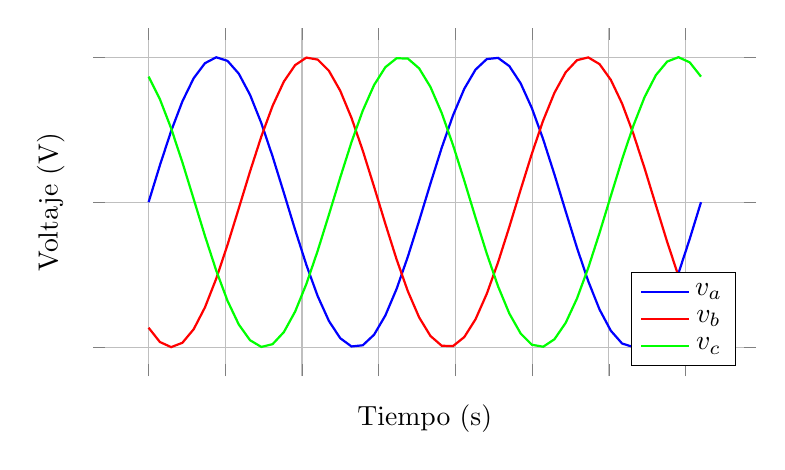
\begin{tikzpicture}
    \begin{axis}[
        width=10cm,
        height=6cm,
        xlabel={Tiempo (s)},
        ylabel={Voltaje (V)},
        legend entries={$v_a$, $v_b$, $v_c$},
        grid=major,  
        legend pos=south east,
        samples=50,
        domain=0:2*360,
        axis line style={draw=none},  % Elimina el recuadro exterior
        xticklabels=\empty,  % Elimina las marcas en el eje x
        yticklabels=\empty,  % Elimina las marcas en el eje y
    ]
    \addplot[blue, thick, domain=0:2*360] {sin(x)};
    \addplot[red, thick, domain=0:2*360] {sin(x - 120)};
    \addplot[green, thick, domain=0:2*360] {sin(x - 240)};
    \end{axis}
    \end{tikzpicture}
    \caption{Sistema trifásico representado en el tiempo}
\end{figure}

Todas las ecuaciones se pueden definir a partir de este modelo, pero se vuelve muy poco práctico para análisis más complejos. Se introduce una forma de representar estas formas de onda en el espacio tridimensional ${\rm I\!R^3}$, en el que se escogen los ejes \((a, b, c)\). Lo que debería esperarse ver es una forma tridimensional en el espacio ${\rm I\!R^3}$. Se comienza en \(t = 0\) y se dibuja un punto en las coordenadas \([v_a(0), v_b(0), v_c(0)]\). Luego, se continúa trazando puntos mientras se avanza a lo largo del eje del tiempo. La forma se puede expresar como curva paramétrica como \([v_a(t), v_b(t), v_c(t)]\). Cuando se representa la forma resultante, puede sorprender, ya que es un círculo perfectamente plano. Cabe destacar que el orden de los ejes depende del contexto, y en este trabajo se toma el sistema de referencia mostrado en las siguientes figuras.


\begin{figure}[!ht]
    \centering
    \begin{subfigure}[b]{3cm}
        \centering
        \hspace*{-1.5cm}
        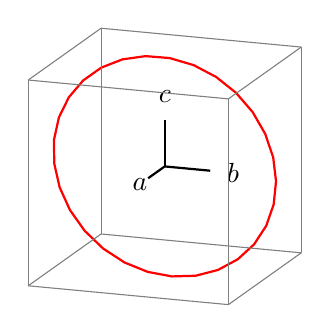
\begin{tikzpicture}
        \begin{axis}[
            %view={-45}{-35},
            view={-20}{-15},
            %view={54.74}{-15},
            axis lines=none,
            xmin=-1.5,
            xmax=1.5,
            ymin=-1.5,
            ymax=1.5,
            zmin=-1.5,
            zmax=1.5,
            no markers,
            axis equal,
            enlargelimits={upper=0.2},
            scale=1,
        ]
        \addplot3+[red, thick, no markers, samples=30, domain=-pi:pi, variable=\t]
            ({sin(deg(\t))}, {sin(deg(\t + 2*pi/3))}, {sin(deg(\t - 2*pi/3))});
        \draw[thick] (axis cs:0, 0, 0) -- (axis cs:0.5, 0, 0) node[pos=1.5]{$b$};
        \draw[thick] (axis cs:0, 0, 0) -- (axis cs:0, 0.5, 0) node[pos=1.5]{$a$};
        \draw[thick] (axis cs:0, 0, 0) -- (axis cs:0, 0, 0.5) node[pos=1.5]{$c$};
        \addplot3[draw=gray, no markers] coordinates {(-1.1, -1.1, -1.1) (-1.1, 1.1, -1.1)};
        \addplot3[draw=gray, no markers] coordinates {(-1.1, 1.1, -1.1) (1.1, 1.1, -1.1)};
        \addplot3[draw=gray, no markers] coordinates {(1.1, 1.1, -1.1) (1.1, -1.1, -1.1)};
        \addplot3[draw=gray, no markers] coordinates {(1.1, -1.1, -1.1) (-1.1, -1.1, -1.1)};
        \addplot3[draw=gray, no markers] coordinates {(-1.1, -1.1, 1.1) (-1.1, 1.1, 1.1)};
        \addplot3[draw=gray, no markers] coordinates {(-1.1, 1.1, 1.1) (1.1, 1.1, 1.1)};
        \addplot3[draw=gray, no markers] coordinates {(1.1, 1.1, 1.1) (1.1, -1.1, 1.1)};
        \addplot3[draw=gray, no markers] coordinates {(1.1, -1.1, 1.1) (-1.1, -1.1, 1.1)};
        \addplot3[draw=gray, no markers] coordinates {(-1.1, -1.1, -1.1) (-1.1, -1.1, 1.1)};
        \addplot3[draw=gray, no markers] coordinates {(-1.1, 1.1, -1.1) (-1.1, 1.1, 1.1)};
        \addplot3[draw=gray, no markers] coordinates {(1.1, 1.1, -1.1) (1.1, 1.1, 1.1)};
        \addplot3[draw=gray, no markers] coordinates {(1.1, -1.1, -1.1) (1.1, -1.1, 1.1)};
        \end{axis}
        \end{tikzpicture}
    \end{subfigure}
    \hfill
    \begin{subfigure}[b]{3cm}
        \centering
            \hspace*{-1.5cm}
            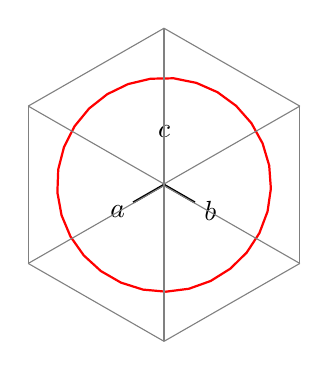
\begin{tikzpicture}
            \begin{axis}[
                view={-45}{-35},
                %view={-20}{-15},
                %view={54.74}{-15},
                axis lines=none,  % Elimina los ejes
                xmin=-.9,
                xmax=.9,
                ymin=-.9,
                ymax=.9,
                zmin=-.9,
                zmax=.9,
                no markers,
                axis equal,
                enlargelimits={upper=0.2},
                scale=1,
            ]
            \addplot3+[red, thick, no markers, samples=30, domain=-pi:pi, variable=\t]
                ({sin(deg(\t))}, {sin(deg(\t + 2*pi/3))}, {sin(deg(\t - 2*pi/3))});
            \draw[thick] (axis cs:0, 0, 0) -- (axis cs:0.5, 0, 0) node[pos=1.5]{$b$};
            \draw[thick] (axis cs:0, 0, 0) -- (axis cs:0, 0.5, 0) node[pos=1.5]{$a$};
            \draw[thick] (axis cs:0, 0, 0) -- (axis cs:0, 0, 0.5) node[pos=1.5]{$c$};
            \addplot3[draw=gray, no markers] coordinates {(-1.1, -1.1, -1.1) (-1.1, 1.1, -1.1)};
            \addplot3[draw=gray, no markers] coordinates {(-1.1, 1.1, -1.1) (1.1, 1.1, -1.1)};
            \addplot3[draw=gray, no markers] coordinates {(1.1, 1.1, -1.1) (1.1, -1.1, -1.1)};
            \addplot3[draw=gray, no markers] coordinates {(1.1, -1.1, -1.1) (-1.1, -1.1, -1.1)};
            \addplot3[draw=gray, no markers] coordinates {(-1.1, -1.1, 1.1) (-1.1, 1.1, 1.1)};
            \addplot3[draw=gray, no markers] coordinates {(-1.1, 1.1, 1.1) (1.1, 1.1, 1.1)};
            \addplot3[draw=gray, no markers] coordinates {(1.1, 1.1, 1.1) (1.1, -1.1, 1.1)};
            \addplot3[draw=gray, no markers] coordinates {(1.1, -1.1, 1.1) (-1.1, -1.1, 1.1)};
            \addplot3[draw=gray, no markers] coordinates {(-1.1, -1.1, -1.1) (-1.1, -1.1, 1.1)};
            \addplot3[draw=gray, no markers] coordinates {(-1.1, 1.1, -1.1) (-1.1, 1.1, 1.1)};
            \addplot3[draw=gray, no markers] coordinates {(1.1, 1.1, -1.1) (1.1, 1.1, 1.1)};
            \addplot3[draw=gray, no markers] coordinates {(1.1, -1.1, -1.1) (1.1, -1.1, 1.1)};
            \end{axis}
            \end{tikzpicture}
    \end{subfigure}
    \hfill
    \begin{subfigure}[b]{3cm}
        \centering
        \hspace*{-1.5cm}
        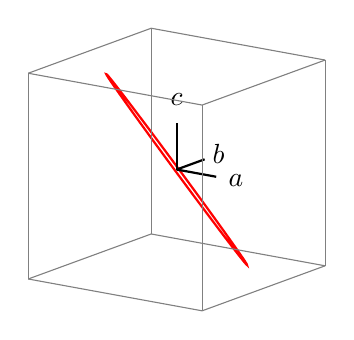
\begin{tikzpicture}
        \begin{axis}[
            %view={-45}{-35},
            %view={-20}{-15},
            view={54.7356103}{-15},
            axis lines=none,
            xmin=-1.5,
            xmax=1.5,
            ymin=-1.5,
            ymax=1.5,
            zmin=-1.5,
            zmax=1.5,
            no markers,
            axis equal,
            enlargelimits={upper=0.2},
            scale=1,
        ]
        \addplot3+[red, thick, no markers, samples=50, domain=-pi:pi, variable=\t]
            ({sin(deg(\t))}, {sin(deg(\t + 2*pi/3))}, {sin(deg(\t - 2*pi/3))});
        \draw[thick] (axis cs:0, 0, 0) -- (axis cs:0.5, 0, 0) node[pos=1.5]{$b$};
        \draw[thick] (axis cs:0, 0, 0) -- (axis cs:0, 0.5, 0) node[pos=1.5]{$a$};
        \draw[thick] (axis cs:0, 0, 0) -- (axis cs:0, 0, 0.5) node[pos=1.5]{$c$};
        \addplot3[draw=gray, no markers] coordinates {(-1.1, -1.1, -1.1) (-1.1, 1.1, -1.1)};
        \addplot3[draw=gray, no markers] coordinates {(-1.1, 1.1, -1.1) (1.1, 1.1, -1.1)};
        \addplot3[draw=gray, no markers] coordinates {(1.1, 1.1, -1.1) (1.1, -1.1, -1.1)};
        \addplot3[draw=gray, no markers] coordinates {(1.1, -1.1, -1.1) (-1.1, -1.1, -1.1)};
        \addplot3[draw=gray, no markers] coordinates {(-1.1, -1.1, 1.1) (-1.1, 1.1, 1.1)};
        \addplot3[draw=gray, no markers] coordinates {(-1.1, 1.1, 1.1) (1.1, 1.1, 1.1)};
        \addplot3[draw=gray, no markers] coordinates {(1.1, 1.1, 1.1) (1.1, -1.1, 1.1)};
        \addplot3[draw=gray, no markers] coordinates {(1.1, -1.1, 1.1) (-1.1, -1.1, 1.1)};
        \addplot3[draw=gray, no markers] coordinates {(-1.1, -1.1, -1.1) (-1.1, -1.1, 1.1)};
        \addplot3[draw=gray, no markers] coordinates {(-1.1, 1.1, -1.1) (-1.1, 1.1, 1.1)};
        \addplot3[draw=gray, no markers] coordinates {(1.1, 1.1, -1.1) (1.1, 1.1, 1.1)};
        \addplot3[draw=gray, no markers] coordinates {(1.1, -1.1, -1.1) (1.1, -1.1, 1.1)};
        \end{axis}
        \end{tikzpicture}
    \end{subfigure}   
    \centering
    \caption{Sistema trifásico representado en el Espacio Vectorial}
\end{figure}


Se puede observar que el sistema trifásico, cuando está equilibrado, se puede representar con solo dos variables, ya que la forma resultante es bidimensional. Se explorará cómo simplificar esto para facilitar el control del PMSM.

\subsection{Transformadas}

Se puede sospechar que lo que se necesita para representar el sistema trifásico con dos variables es un cambio de base, en particular, una rotación. El enfoque general sería utilizar la transformada de Concordia. La transformada de Clarke es el caso particular para 3 dimensiones de la transformada de Concordia, que se utiliza para cualquier número de dimensiones.

Se pueden encontrar dos transformadas de Clarke: la transformada de Clarke ortonormal y la transformada de Clarke de amplitud constante o módulo invariante. Además, se pueden considerar el eje $\alpha$ avanzado 90º respecto al eje $\beta$, o viceversa. Para el análisis y control de una máquina eléctrica se suele utilizar la transformada de Clarke de amplitud constante con $\alpha$ avanzada.

\subsubsection{Transformada de Clarke ortonormal}

Esta transformada se utiliza cuando la potencia del sistema debe permanecer inalterada después de la transformación. Se aplican dos rotaciones al marco de referencia $abc$ y se crea el marco de referencia $\alpha\beta\gamma$. En este nuevo marco de referencia, la trayectoria del vector espacial está completamente contenida en el plano $\alpha\beta$ cuando el sistema está equilibrado, y el eje $\gamma$ se utiliza para explicar el componente homopolar del sistema (la suma de los tres componentes debe ser igual a 0 si el sistema está equilibrado, de lo contrario, aparece el componente homopolar).


\begin{figure}[!ht]
    \centering
    \begin{subfigure}[b]{3cm}
        \centering
        \hspace*{-1.5cm}
        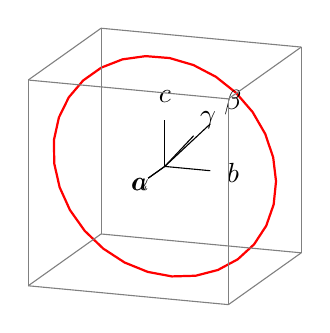
\begin{tikzpicture}
        \begin{axis}[
            %view={-45}{-35},
            view={-20}{-15},
            %view={54.74}{-15},
            axis lines=none,
            xmin=-1.5,
            xmax=1.5,
            ymin=-1.5,
            ymax=1.5,
            zmin=-1.5,
            zmax=1.5,
            no markers,
            axis equal,
            enlargelimits={upper=0.2},
            scale=1,
        ]
        \addplot3+[red, thick, no markers, samples=30, domain=-pi:pi, variable=\t]
            ({sin(deg(\t))}, {sin(deg(\t + 2*pi/3))}, {sin(deg(\t - 2*pi/3))});
        \draw (axis cs:0, 0, 0) -- (axis cs:0.5, 0, 0) node[pos=1.5]{$b$};
        \draw (axis cs:0, 0, 0) -- (axis cs:0, 0.5, 0) node[pos=1.5]{$a$};
        \draw (axis cs:0, 0, 0) -- (axis cs:0, 0, 0.5) node[pos=1.5]{$c$};
        \draw (axis cs:0, 0, 0) -- (axis cs:0.5, 0, 0.5) node[pos=1.5]{$\beta$};
        \draw (axis cs:0, 0, 0) -- (axis cs:0, 0.5, 0) node[pos=1.5]{$\alpha$};
        \draw (axis cs:0, 0, 0) -- (axis cs:0.5, 0.5, 0.5) node[pos=1.5]{$\gamma$};
        
        \addplot3[draw=gray, no markers] coordinates {(-1.1, -1.1, -1.1) (-1.1, 1.1, -1.1)};
        \addplot3[draw=gray, no markers] coordinates {(-1.1, 1.1, -1.1) (1.1, 1.1, -1.1)};
        \addplot3[draw=gray, no markers] coordinates {(1.1, 1.1, -1.1) (1.1, -1.1, -1.1)};
        \addplot3[draw=gray, no markers] coordinates {(1.1, -1.1, -1.1) (-1.1, -1.1, -1.1)};
        \addplot3[draw=gray, no markers] coordinates {(-1.1, -1.1, 1.1) (-1.1, 1.1, 1.1)};
        \addplot3[draw=gray, no markers] coordinates {(-1.1, 1.1, 1.1) (1.1, 1.1, 1.1)};
        \addplot3[draw=gray, no markers] coordinates {(1.1, 1.1, 1.1) (1.1, -1.1, 1.1)};
        \addplot3[draw=gray, no markers] coordinates {(1.1, -1.1, 1.1) (-1.1, -1.1, 1.1)};
        \addplot3[draw=gray, no markers] coordinates {(-1.1, -1.1, -1.1) (-1.1, -1.1, 1.1)};
        \addplot3[draw=gray, no markers] coordinates {(-1.1, 1.1, -1.1) (-1.1, 1.1, 1.1)};
        \addplot3[draw=gray, no markers] coordinates {(1.1, 1.1, -1.1) (1.1, 1.1, 1.1)};
        \addplot3[draw=gray, no markers] coordinates {(1.1, -1.1, -1.1) (1.1, -1.1, 1.1)};
        \end{axis}
        \end{tikzpicture}
    \end{subfigure}
    \hfill
    \begin{subfigure}[b]{3cm}
        \centering
            \hspace*{-1.5cm}
            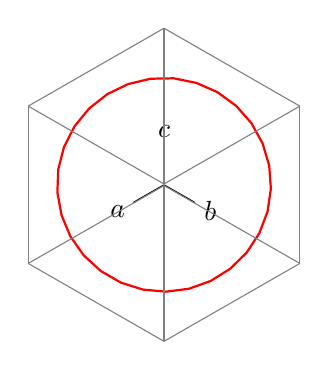
\begin{tikzpicture}
            \begin{axis}[
                view={-45}{-35},
                %view={-20}{-15},
                %view={54.74}{-15},
                axis lines=none,  % Elimina los ejes
                xmin=-.9,
                xmax=.9,
                ymin=-.9,
                ymax=.9,
                zmin=-.9,
                zmax=.9,
                no markers,
                axis equal,
                enlargelimits={upper=0.2},
                scale=1,
            ]
            \addplot3+[red, thick, no markers, samples=30, domain=-pi:pi, variable=\t]
                ({sin(deg(\t))}, {sin(deg(\t + 2*pi/3))}, {sin(deg(\t - 2*pi/3))});
            \draw (axis cs:0, 0, 0) -- (axis cs:0.5, 0, 0) node[pos=1.5]{$b$};
            \draw (axis cs:0, 0, 0) -- (axis cs:0, 0.5, 0) node[pos=1.5]{$a$};
            \draw (axis cs:0, 0, 0) -- (axis cs:0, 0, 0.5) node[pos=1.5]{$c$};
            \addplot3[draw=gray, no markers] coordinates {(-1.1, -1.1, -1.1) (-1.1, 1.1, -1.1)};
            \addplot3[draw=gray, no markers] coordinates {(-1.1, 1.1, -1.1) (1.1, 1.1, -1.1)};
            \addplot3[draw=gray, no markers] coordinates {(1.1, 1.1, -1.1) (1.1, -1.1, -1.1)};
            \addplot3[draw=gray, no markers] coordinates {(1.1, -1.1, -1.1) (-1.1, -1.1, -1.1)};
            \addplot3[draw=gray, no markers] coordinates {(-1.1, -1.1, 1.1) (-1.1, 1.1, 1.1)};
            \addplot3[draw=gray, no markers] coordinates {(-1.1, 1.1, 1.1) (1.1, 1.1, 1.1)};
            \addplot3[draw=gray, no markers] coordinates {(1.1, 1.1, 1.1) (1.1, -1.1, 1.1)};
            \addplot3[draw=gray, no markers] coordinates {(1.1, -1.1, 1.1) (-1.1, -1.1, 1.1)};
            \addplot3[draw=gray, no markers] coordinates {(-1.1, -1.1, -1.1) (-1.1, -1.1, 1.1)};
            \addplot3[draw=gray, no markers] coordinates {(-1.1, 1.1, -1.1) (-1.1, 1.1, 1.1)};
            \addplot3[draw=gray, no markers] coordinates {(1.1, 1.1, -1.1) (1.1, 1.1, 1.1)};
            \addplot3[draw=gray, no markers] coordinates {(1.1, -1.1, -1.1) (1.1, -1.1, 1.1)};
            \end{axis}
            \end{tikzpicture}
    \end{subfigure}
    \hfill
    \begin{subfigure}[b]{3cm}
        \centering
        \hspace*{-1.5cm}
        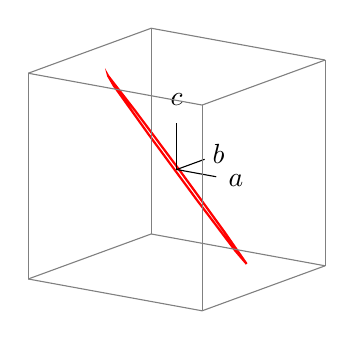
\begin{tikzpicture}
        \begin{axis}[
            %view={-45}{-35},
            %view={-20}{-15},
            view={54.74}{-15},
            axis lines=none,
            xmin=-1.5,
            xmax=1.5,
            ymin=-1.5,
            ymax=1.5,
            zmin=-1.5,
            zmax=1.5,
            no markers,
            axis equal,
            enlargelimits={upper=0.2},
            scale=1,
        ]
        \addplot3+[red, thick, no markers, samples=10, domain=-pi:pi, variable=\t]
            ({sin(deg(\t))}, {sin(deg(\t + 2*pi/3))}, {sin(deg(\t - 2*pi/3))});
        \draw (axis cs:0, 0, 0) -- (axis cs:0.5, 0, 0) node[pos=1.5]{$b$};
        \draw (axis cs:0, 0, 0) -- (axis cs:0, 0.5, 0) node[pos=1.5]{$a$};
        \draw (axis cs:0, 0, 0) -- (axis cs:0, 0, 0.5) node[pos=1.5]{$c$};

        \addplot3[draw=gray, no markers] coordinates {(-1.1, -1.1, -1.1) (-1.1, 1.1, -1.1)};
        \addplot3[draw=gray, no markers] coordinates {(-1.1, 1.1, -1.1) (1.1, 1.1, -1.1)};
        \addplot3[draw=gray, no markers] coordinates {(1.1, 1.1, -1.1) (1.1, -1.1, -1.1)};
        \addplot3[draw=gray, no markers] coordinates {(1.1, -1.1, -1.1) (-1.1, -1.1, -1.1)};
        \addplot3[draw=gray, no markers] coordinates {(-1.1, -1.1, 1.1) (-1.1, 1.1, 1.1)};
        \addplot3[draw=gray, no markers] coordinates {(-1.1, 1.1, 1.1) (1.1, 1.1, 1.1)};
        \addplot3[draw=gray, no markers] coordinates {(1.1, 1.1, 1.1) (1.1, -1.1, 1.1)};
        \addplot3[draw=gray, no markers] coordinates {(1.1, -1.1, 1.1) (-1.1, -1.1, 1.1)};
        \addplot3[draw=gray, no markers] coordinates {(-1.1, -1.1, -1.1) (-1.1, -1.1, 1.1)};
        \addplot3[draw=gray, no markers] coordinates {(-1.1, 1.1, -1.1) (-1.1, 1.1, 1.1)};
        \addplot3[draw=gray, no markers] coordinates {(1.1, 1.1, -1.1) (1.1, 1.1, 1.1)};
        \addplot3[draw=gray, no markers] coordinates {(1.1, -1.1, -1.1) (1.1, -1.1, 1.1)};
        \end{axis}
        \end{tikzpicture}
    \end{subfigure}   
    \centering
    \caption{Sistema trifásico representado en el Espacio Vectorial}
\end{figure}


No se derivará la transformada aquí, aunque es necesario comprender lo que hace y conocer la matriz de transformación.

Lo que hace la transformada es colocar dos de los ejes del sistema de referencia en el plano formado por el círculo generado por el vector espacial. El eje restante es perpendicular a ese plano y representa el componente homopolar.

A continuación se presenta la forma matricial de la transformada:

\begin{equation}
\begin{bmatrix}
    \alpha \\
    \beta \\
    \gamma
\end{bmatrix}
=
\sqrt{\frac{2}{3}}
\begin{bmatrix}
    1 & -\frac{1}{2} & -\frac{1}{2} \\
    0 & \frac{\sqrt{3}}{2} & -\frac{\sqrt{3}}{2} \\
    \frac{1}{\sqrt{2}} & \frac{1}{\sqrt{2}} & \frac{1}{\sqrt{2}}
\end{bmatrix}
\begin{bmatrix}
    a \\
    b \\
    c
\end{bmatrix}
\end{equation}

La forma matricial de la transformada inversa es:

\begin{equation}
\begin{bmatrix}
    a \\
    b \\
    c
\end{bmatrix}
=
\sqrt{\frac{2}{3}}
\begin{bmatrix}
    1 & 0 & \frac{1}{\sqrt{2}} \\
    -\frac{1}{2} & \frac{\sqrt{3}}{2} & \frac{1}{\sqrt{2}} \\
    -\frac{1}{2} & -\frac{\sqrt{3}}{2} & \frac{1}{\sqrt{2}}
\end{bmatrix}
\begin{bmatrix}
    \alpha \\
    \beta \\
    \gamma
\end{bmatrix}
\end{equation}

Esta transformada tiene la particularidad de mantener constante la potencia del sistema, de modo que se cumple la siguiente condición:

\begin{equation}
p(t) = p_{abc} = p_{\alpha\beta\gamma, \text{ortonormal}} = v_a \cdot i_a + v_b \cdot i_b + v_c \cdot i_c = v_\alpha \cdot i_\alpha + v_\beta \cdot i_\beta + v_\gamma \cdot i_\gamma
\end{equation}

\subsubsection{Transformada de Clarke de Amplitud Constante}

Mantener constante la potencia a lo largo de las transformadas puede ser útil en algunos contextos, pero lo que se suele implementar es una variante de la transformada de Clarke que mantiene constante la amplitud de la magnitud.

La transformada no es ortonormal, ya que ajusta las magnitudes para que el módulo de las variables sea el adecuado, pero la rotación se mantiene igual.

\begin{equation}
\begin{bmatrix}
    \alpha' \\
    \beta' \\
    \gamma'
\end{bmatrix}
=
\frac{2}{3}
\begin{bmatrix}
    1 & -\frac{1}{2} & -\frac{1}{2} \\
    0 & \frac{\sqrt{3}}{2} & -\frac{\sqrt{3}}{2} \\
    \frac{1}{2} & \frac{1}{2} & \frac{1}{2}
\end{bmatrix}
\begin{bmatrix}
    a \\
    b \\
    c
\end{bmatrix}
\end{equation}

La transformada inversa es la siguiente:

\begin{equation}
\begin{bmatrix}
    a \\
    b \\
    c
\end{bmatrix}
=
\begin{bmatrix}
    1 & 0 & 1 \\
    -\frac{1}{2} & \frac{\sqrt{3}}{2} & 1 \\
    -\frac{1}{2} & -\frac{\sqrt{3}}{2} & 1
\end{bmatrix}
\begin{bmatrix}
    \alpha' \\
    \beta' \\
    \gamma'
\end{bmatrix}
\end{equation}

Se puede derivar que:

\begin{equation}
p_{abc} = \frac{3}{2} \cdot (v_{\alpha'} \cdot i_{\alpha'} + v_{\beta'} \cdot i_{\beta'} + v_{\gamma'} \cdot i_{\gamma'})
\end{equation}


\subsubsection{Transformada de Park}

Después de aplicar la transformada de Clarke, todavía quedan dos variables sinusoidales (\(\alpha\beta\) si se considera \(\gamma = 0\)), lo que dificulta el análisis para que el control sea sencillo. Por lo tanto, se aplica otra transformada para convertir estas cantidades sinusoidales en constantes.

Ahora, considerando que el vector espacial gira a una velocidad de \(\omega = 2\pi f\), si se aplica continuamente una rotación alrededor del eje \(\gamma\) con un ángulo \(\theta = \omega  t\), se puede representar el vector espacial como una composición de dos variables continuas (en lugar de sinusoides). Además, si se sincroniza esta rotación con el ángulo del vector espacial (el eje \(d\) apuntando al vector espacial), se obtiene una variable continua (\(d\)) y una segunda variable de valor nulo (\(q\)).

\begin{figure}[!ht]
  \centering
  %\includegraphics[width=0.5\textwidth]{ruta_de_la_imagen_en_formato_latex}
  \caption{Transformada de Park.}
\end{figure}

Se puede ver que la transformada es simplemente una rotación a lo largo de uno de los ejes de la base:

\begin{equation}
\begin{bmatrix}
    d \\
    q \\
    0
\end{bmatrix}
=
\begin{bmatrix}
    \cos(\theta) & \sin(\theta) & 0 \\
    -\sin(\theta) & \cos(\theta) & 0 \\
    0 & 0 & 1
\end{bmatrix}
\begin{bmatrix}
    \alpha \\
    \beta \\
    \gamma
\end{bmatrix}
\end{equation}

%% DESDE AQUI TRACUCCION POCHA DE LA WIKI --> REVISAR TODAS LAS EQs!!!!!!!!!!!
\subsection{Modelo \textit{dq0} del PMSM}

En esta sección, se convertirá el modelo trifásico inicial del PMSM en un modelo continuo en el marco de referencia $d - q$. Antes, se omitieron las ecuaciones del modelo trifásico, pero utilizando estas y aplicando las transformadas de Clarke y Park, se obtienen las ecuaciones que se derivarán en esta sección.

El enfoque general es utilizar la transformada de amplitud constante, lo que lleva a estas ecuaciones para las tensiones y corrientes del estator:

\begin{equation}
	\begin{bmatrix}
		v_d \\
		v_q \\
		v_0
	\end{bmatrix}
	=
	\begin{bmatrix}
		\cos(\theta) & \sin(\theta) & 0  \\
		-\sin(\theta) & \cos(\theta) & 0  \\
		0 & 0 & 1
	\end{bmatrix}
	\frac{2}{3}
	\begin{bmatrix}
		1 & -\frac{1}{2} & -\frac{1}{2} \\
		0 & \frac{\sqrt{3}}{2} & -\frac{\sqrt{3}}{2} \\
		\frac{1}{2} & \frac{1}{2} & \frac{1}{2}
	\end{bmatrix}
	\begin{bmatrix}
		v_a \\
		v_b \\
		v_c
	\end{bmatrix}
\end{equation}

\begin{equation}
	\begin{bmatrix}
		i_d \\
		i_q \\
		i_0
	\end{bmatrix}
	=
	\begin{bmatrix}
		\cos(\theta) & \sin(\theta) & 0  \\
		-\sin(\theta) & \cos(\theta) & 0  \\
		0 & 0 & 1
	\end{bmatrix}
	\frac{2}{3}
	\begin{bmatrix}
		1 & -\frac{1}{2} & -\frac{1}{2} \\
		0 & \frac{\sqrt{3}}{2} & -\frac{\sqrt{3}}{2} \\
		\frac{1}{2} & \frac{1}{2} & \frac{1}{2}
	\end{bmatrix}
	\begin{bmatrix}
		i_a \\
		i_b \\
		i_c
	\end{bmatrix}
\end{equation}

El modelo de circuito equivalente se divide en los circuitos del eje $d$ y el eje $q$:

\begin{figure}[!ht]
	\centering
	
	% Side-by-side d-q circuits
	\begin{circuitikz}[american voltages]
		% d-axis circuit
		\draw (0,0) to [L, l=$L_d$, o-] ++(2,0) to [R, l=$R_s$] ++(2,0) to [V, v^=$\omega_e\cdot L_q\cdot i_q$, invert] ++(2,0) -- ++(0,-2){};
		% Parallel line
		\draw (0,-2) node[circ, fill=none]{} -- ++(6,0);
		% Current label
		\draw (4,-2) to [open, i_=$i_d$] (2,-2);
		% Voltage labels
		\draw (0,0) to [open, v^=$v_d$] (0,-2);
	\end{circuitikz}
	\hspace{1cm} % Adjust the horizontal space between circuits
	\begin{circuitikz}[american voltages]
		% q-axis circuit
		\draw (0,0) to [L, l=$L_q$, o-] ++(2,0) to [R, l=$R_s$] ++(2,0) to [V, v^=$\omega_e\cdot L_d\cdot i_d$] ++(2,0) to [V, v^=$\omega_e \lambda_m$] ++(0,-2){};
		% Parallel line
		\draw (0,-2) node[circ, fill=none]{} -- ++(6,0);
		% Current label
		\draw (4,-2) to [open, i_=$i_q$] (2,-2);
		% Voltage labels
		\draw (0,0) to [open, v^=$v_q$] (0,-2);
	\end{circuitikz}
	
	\caption{Circuitos eléctricos equivalentes del modelo $d-q$ de un PMSM.}
\end{figure}

Se puede observar que:

\begin{equation}
v_d = v_{r_s} - \omega_e \cdot L_q \cdot i_q + v_{L_d}
\end{equation}

\begin{equation}
v_d = r_s\cdot i_d - \omega_e \cdot L_q \cdot i_q + L_d\cdot\frac{d i_d}{d t}
\end{equation}

Y:

\begin{equation}
v_q = v_{r_s} - \omega_e \cdot L_d \cdot i_d + \omega_e \cdot \lambda_m + v_{L_q}
\end{equation}

\begin{equation}
v_q = r_s\cdot i_q - \omega_e \cdot L_d \cdot i_q + \omega_e \cdot \lambda_m + L_q\cdot\frac{d i_q}{d t}
\end{equation}

Donde:
\begin{itemize}
    \item \(v_d\) y \(v_q\) son las tensiones en los ejes d y q respectivamente.
    \item \(i_d\) y \(i_q\) son las corrientes en los ejes d y q respectivamente.
    \item \(L_d\) y \(L_q\) son las inductancias en los ejes d y q respectivamente.
    \item \(\omega_e\) es la velocidad eléctrica, que es la velocidad mecánica multiplicada por el número de pares de polos del PMSM (\(\omega_e = \omega_m \cdot pp = \omega_m \cdot \frac{n}{2}\)).
    \item \(\lambda_m\) es el flujo magnético generado por los imanes permanentes. La magnitud del flujo magnético generado afecta directamente la magnitud de la tensión inducida en las fases del estator. Este parámetro se puede transformar fácilmente en \(k_E\), que es la relación entre la velocidad mecánica del rotor y la tensión generada en las 3 fases.
\end{itemize}


Hay PMSM cuyos imanes están montados dentro del rotor (IPM) y otros cuyos imanes están en la superficie del rotor (SPM). Esta diferenciación juega un papel importante en el desarrollo del modelo y el control, porque en los SPM se cumple \(L_d = L_q\), a menudo escrito solo como \(L\). Además, si se trata de un IPM, la orientación de los imanes puede cambiar las trayectorias del control, de manera que si son imanes tangenciales se da \(L_d > L_q\) y si son imanes radiales \(L_d < L_q\). Se desarrollarán las ecuaciones para motores IPM, pero se ha de tener en cuenta que se pueden realizar muchas simplificaciones si el motor es un SPM. Una situación que se dará es que algunas ecuaciones tienen alguna forma de \(L_d - L_q\) como denominador, lo cual es bastante problemático si se está tratando de implementar la ecuación directamente. Por ese motivo, es mejor diferenciar las el tipo de motor antes de implementar las ecuaciones. Una solución válida es tener en cuenta la anisotropía magnética que suelen presentar la mayoría de SPMs, con lo que \(L_d < L_q\) y se pueden aplicar las ecuaciones del IPM.

************FIGURA TIPOS DE MOTORES*******************

La potencia eléctrica se define como:

\begin{equation}
p_e = \frac{3}{2}\cdot(v_d i_d + v_q i_q)
\end{equation}

Si se supone que la máquina es perfectamente eficiente, se puede decir que la potencia mecánica es igual a la potencia eléctrica, \(p_e = p_m\). Sabiendo que \(p_m = \omega_m T_{em}\), donde \(T_{em}\) es el par electromagnético producido, se puede derivar:

\begin{equation}
T_{em} = \frac{3}{2\cdot \omega_m}\cdot(v_d i_d + v_q i_q) = \frac{3}{2\cdot \omega_e}\frac{n}{2}\cdot(v_d i_d + v_q i_q)
\end{equation}

\begin{equation}
T_{em} = \frac{3}{2}\frac{n}{2}\cdot((L_d - L_q) i_q i_d + \lambda_m i_q)
\end{equation}

También se puede establecer un límite de voltaje, porque el PMSM generalmente se controla con un inversor de fuente de voltaje (VSI) modulado por SVPWM y la tensión de salida está limitada a \(\frac{V_{DC}}{\sqrt{3}}\). En esta ecuación, no se considera la caída de tensión por la resistencia del estator \(R_s\), ya que haría que las ecuaciones fueran muy densas y el efecto de esta caída de voltaje es despreciable a altas velocidades.

\begin{equation}
\left(\frac{\frac{V_{DC}}{\sqrt{3}}}{\omega_e}\right)^2 \geq \left(\frac{\lambda_m}{L_d}+i_d\right)^2+(L_q+i_q)^2
\end{equation}

\subsection{Curvas características del PMSM}

Las ecuaciones del PMSM son muy útiles cuando se diseña el control y la implementación real, pero antes de eso, es muy recomendable verlas en un gráfico para comprender mejor algunas de las intuiciones detrás de ellas.

\subsubsection{Curva de par-velocidad y potencia-velocidad}

Las primeras curvas estudiadas son las de par-velocidad y potencia-velocidad. Definen la intención de diseño del PMSM, ilustrando el rendimiento deseado. El objetivo al diseñar el control es tratar de igualar o incluso superar estas curvas.


\begin{figure}[!ht]
    \centering
    \hspace*{-1.5cm}
    \begin{tikzpicture}
    \begin{axis}[
        axis lines=middle,
        width=10cm,
        height=8cm,
        x label style={at={(axis description cs:-0.1,0.5)},anchor=north},
        y label style={at={(axis description cs:0.5,-0.1)},rotate=90,anchor=south},
        xlabel={$\omega_m$},
        ylabel={$T_{em}$},
        ytick={-26, 26},
        xtick={-2000,-1000,1000,2000},
        yticklabels={$-T_{em,max}$, $T_{em,max}$},
        xticklabels={$-\omega_{m,max}$, $-\omega_{m,nom}$, $\omega_{m,nom}$,$\omega_{m,max}$},
        grid=none,  
        ymin=-40,
        ymax=40,
        samples=15,
        domain=-2500:2500,
        nodes near coords align={south east},
        y tick label style={yshift={sign(\tick)*10}},
        ylabel style={rotate=-90},
        %no marks
        % axis line style={draw=none},  % Elimina el recuadro exterior
    ]
    \addplot[blue, thick, domain=-1000:1000] {26};
    \addplot[blue, thick, domain=-1000:1000] {-26};
    \addplot[blue, thick, domain=1000:2500] {26000/x};
    \addplot[blue, thick, domain=-2500:-1000] {-26000/x};
    \addplot[white, line width=1mm, domain=2000:2500] {26000/x};
    \addplot[white, line width=1mm, domain=-2500:-2000] {-26000/x};
    \addplot[blue, thick, domain=1000:2500] {-26000/x};
    \addplot[blue, thick, domain=-2500:-1000] {26000/x};
    \addplot[white, line width=1mm, domain=2000:2500] {-26000/x};
    \addplot[white, line width=1mm, domain=-2500:-2000] {26000/x};
    \end{axis}
    \end{tikzpicture}
    \caption{Curva de par-velocidad del PMSM.}
\end{figure}


La curva es una función por tramos, que toma \(T_{em,max}\), \(\omega_{m,max}\) y \(P_{m,max}\) como sus parámetros.

La curva es constante desde \(\omega_m = 0\) hasta \(\omega_m = \omega_{m,nom} = \frac{P_{m,max}}{T_{em,max}}\), donde su valor es \(T_{em,max}\). Esta porción es lo que se conoce como la zona de par constante. Desde \(\omega_m = \omega_{m,nom}\) hasta \(\omega_m = \omega_{m,max}\), \(T_{em}\) se define como \(T_{em} = \frac{P_{m,max}}{\omega_m}\), lo que da una curva de tipo \(y=\frac{a}{x}\). Esto se llama la zona de potencia constante.

\[
T_{em} = 
\begin{cases}
  T_{em,max} & -\omega_{m,nom} < \omega_m < \omega_{m,nom} \\
  -T_{em,max} & -\omega_{m,nom} < \omega_m < \omega_{m,nom} \\
  \frac{P_{m,max}}{\omega_m} & \omega_{m,nom}\leq \omega_m\leq \omega_{m,max} (T_{em,max}),-\omega_{m,max}\leq \omega_m\leq -\omega_{m,nom} (-T_{em,max})\\
  -\frac{P_{m,max}}{\omega_m} & \omega_{m,nom}\leq \omega_m\leq \omega_{m,max} (-T_{em,max}),-\omega_{m,max}\leq \omega_m\leq -\omega_{m,nom} (T_{em,max})
\end{cases}
\]

Además \(P_m\) aumentará linealmente con \(\omega_m\) hasta \(\omega_{m,nom}\), ya que \(P_m = T_{em} \cdot \omega_m\). Desde \(\omega_{m,nom}\) hasta \(\omega_{m,max}\), \(P_m\) es una recta de valor \(P_{m,max}\)

\subsubsection{CLC (Círculo de límite de corriente)}

Es obvio que la corriente eléctrica suministrada al PMSM debe estar limitada. Por lo general, el fabricante del motor establecerá la corriente alterna máxima, lo cual se traduce en un límite para \(i_d\) y \(i_q\).

A continuación, se presenta un gráfico muy útil para conocer los límites del motor. Se establecen los ejes como $i_d$ e $i_q$. Por ejemplo, si un motor está funcionando con $i_d = -1 \, \text{A}$ e $i_q = 5 \, \text{A}$, se dibuja un punto en $(-1,5)$. Como se puede apreciar, este es un sistema de coordenadas cartesianas. También puede convertirse en un sistema de coordenadas polares, que utiliza una magnitud y un ángulo. La magnitud del vector será entonces:
\begin{equation}
I_{s} = \sqrt{i_d^2+i_q^2} [\text{A}]
\end{equation}

Y el ángulo:

\begin{equation}
\gamma = \arctan\left(\frac{i_q}{i_d}\right) [\text{rad}]
\end{equation}

Se puede observar que la corriente máxima puede expresarse más fácilmente como $I_s$, independientemente del ángulo $\gamma$ (no debe confundirse con el $\gamma$ de la transformada de Clarke). Por lo tanto, se puede representar $I_s = I_{s,\text{max}} , \forall \gamma \in [0,2\pi]$

\begin{figure}[!ht]
	\centering
	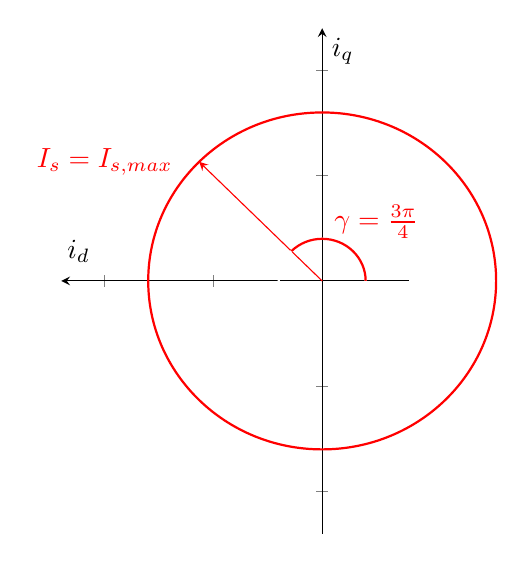
\begin{tikzpicture}
		\begin{axis}[
			axis lines=middle,
			width=6cm,
			height=8cm,
			xlabel={$i_d$},
			x label style={at={(axis description cs:0.05,0.6)},anchor=north},
			ylabel={$i_q$},
			grid=none,
			xmin=-1.2,
			xmax=0.4,
			ymin=-1.2,
			ymax=1.2,
			no markers,
			x axis line style={stealth-},
			xticklabels=\empty,
			yticklabels=\empty,
			clip=false,          % Disable clipping
			]
			
			% Límite de corriente Is_max
			\draw[red, thick] (0,0) circle [radius=0.8];
			\draw [red, -stealth](0,0) -- (-0.56568542494,0.56568542494) node at (-1,0.56568542494) {$I_s = I_{s,\text{max}}$};
			\draw [white, thick] (axis cs: 0.2, 0) arc (0:180:0.2);
			\draw [red, thick] (axis cs: 0.2, 0) arc (0:135:0.2);
			\node[red] at (axis cs: 0.25, 0.28) {$\gamma = \frac{3\pi}{4}$};
			
		\end{axis}
	\end{tikzpicture}
  \caption{Círculo de límite de corriente.}
\end{figure}


Resulta ser un círculo, lo cual tiene sentido, ya que es un vector de magnitud constante. Además, el vector de corriente $I_s\angle \gamma = I_{s,\text{max}} \angle{\frac{3\pi}{4}}$ se representa para facilitar su comprensión.


\subsubsection{TH (Hipérbolas de par)}

Si se estudia la ecuación del par, es evidente que \(T_{em}\) es una función de \((i_d, i_q)\). El resto de parámetros son constantes, por lo que se puede establecer un valor fijo de par y deslizar alrededor de \((i_d, i_q)\) para generar una curva. La forma de la curva resultante es una hipérbola.

\begin{equation}
T_{em} = \frac{3}{2}pp\cdot((L_d - L_q)\cdot I_s^2 \cdot \sin(\gamma)\cos(\gamma) + \lambda_m\cdot I_s\cdot \sin(\gamma))
\end{equation}




\begin{figure}[!ht]
  \centering
    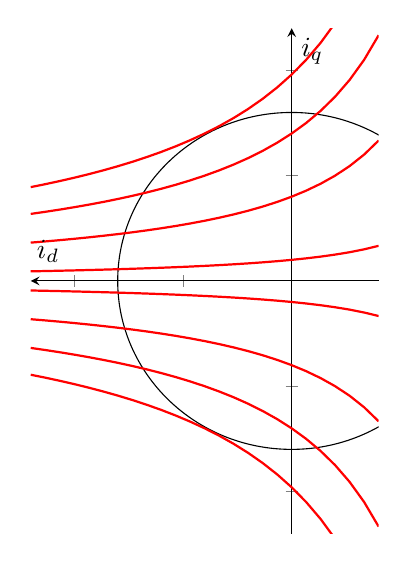
\begin{tikzpicture}
    \begin{axis}[
        axis lines=middle,
        width=6cm,
        height=8cm,
        xlabel={$i_d$},
        x label style={at={(axis description cs:0.05,0.6)},anchor=north},
        ylabel={$i_q$},
        %y label style={at={(axis description cs:0.95,0.05}},
        grid=none,
        xmin=-1.2,
        xmax=0.4,
        ymin=-1.2,
        ymax=1.2,
        no markers,
        x axis line style = {stealth-},
        xticklabels=\empty,  % Elimina las marcas en el eje x
        yticklabels=\empty,  % Elimina las marcas en el eje y
    ]
    
    \draw[black] (0,0) circle [radius=0.8];
    \addplot[red, thick, domain=-1.2:0.4] {4*0.1/(3*2*((2/3)+(2/3)/1*(1-2)*x))};
    \addplot[red, thick, domain=-1.2:0.4] {4*0.4/(3*2*((2/3)+(2/3)/1*(1-2)*x))};
    \addplot[red, thick, domain=-1.2:0.4] {4*0.7/(3*2*((2/3)+(2/3)/1*(1-2)*x))};
    \addplot[red, thick, domain=-1.2:0.4] {4*0.98/(3*2*((2/3)+(2/3)/1*(1-2)*x))};
    
    \addplot[red, thick, domain=-1.2:0.4] {-4*0.1/(3*2*((2/3)+(2/3)/1*(1-2)*x))};
    \addplot[red, thick, domain=-1.2:0.4] {-4*0.4/(3*2*((2/3)+(2/3)/1*(1-2)*x))};
    \addplot[red, thick, domain=-1.2:0.4] {-4*0.7/(3*2*((2/3)+(2/3)/1*(1-2)*x))};
    \addplot[red, thick, domain=-1.2:0.4] {-4*0.98/(3*2*((2/3)+(2/3)/1*(1-2)*x))};
    

    \end{axis}
    \end{tikzpicture}
  \caption{Hipérbolas de par.}
\end{figure}


El gráfico se limita a los cuadrantes 2 y 3 por un motivo ilustrado con estas hipérbolas: solo los valores negativos de \(i_d\) contribuyen a la generación de par. Cuando \(i_d>0\), se necesita más corriente para generar la misma cantidad de par. Cuanto más alejada está la hipérbole del eje \(i_d\), más par representa en valor absoluto. Aquellas hipérbolas que quedan por encima del eje \(i_d\), es decir, \(i_q > 0\) son par positivo, mientras que si \(i_q < 0\), el par es de sentido opuesto.

\subsubsection{VLE (Elipses de límite de voltaje)}

Tomando la ecuación de voltaje presentada anteriormente, se puede demostrar que es una elipse. Del mismo modo que con las hipérbolas de par, se pueden establecer una velocidad y una tensión, y deslizar valores de \((i_d, i_q)\) para generar la curva.

\begin{equation}
1 \geq \frac{\left(\frac{\lambda_m}{L_d}+i_d\right)^2}{\left(\frac{\frac{V_{DC}}{\sqrt{3}}}{\omega_e}\right)^2}+\frac{(L_q+i_q)^2}{\left(\frac{\frac{V_{DC}}{\sqrt{3}}}{\omega_e}\right)^2}
\end{equation}




\begin{figure}[!ht]
  \centering
    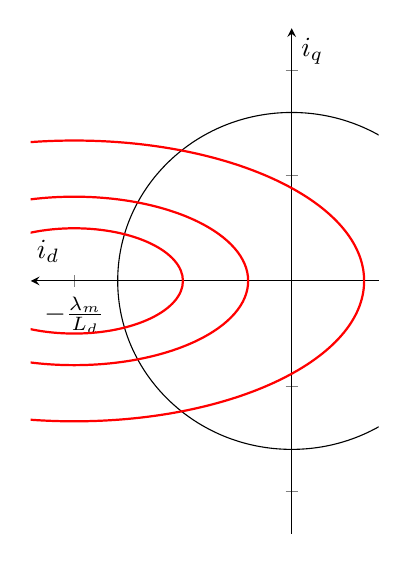
\begin{tikzpicture}
    \begin{axis}[
        axis lines=middle,
        width=6cm,
        height=8cm,
        xlabel={$i_d$},
        x label style={at={(axis description cs:0.05,0.6)},anchor=north},
        ylabel={$i_q$},
        %y label style={at={(axis description cs:0.95,0.05}},
        grid=none,
        xmin=-1.2,
        xmax=0.4,
        ymin=-1.2,
        ymax=1.2,
        no markers,
        x axis line style = {stealth-},
        xtick = {-1},
        xticklabels={$-\frac{\lambda_m}{L_d}$},  % Elimina las marcas en el eje x
        yticklabels=\empty,  % Elimina las marcas en el eje y
    ]
    
    
    \draw[black] (0,0) circle [radius=0.8];
    \draw[red, thick] (-1,0) ellipse (1.333333 and 0.66666666);
    \draw[red, thick] (-1,0) ellipse (0.8 and 0.4);
    \draw[red, thick] (-1,0) ellipse (0.5 and 0.25);

    \end{axis}
    \end{tikzpicture}
  \caption{Elipses de límite de voltaje con $I_{sc} > I_{s,max}$.}
\end{figure}


Al representar estas elipses, normalmente se anotan los valores de velocidad en rpm mecánicas, ya que es mucho más fácil hacerse una idea de los límites del motor junto al resto de curvas (\(\omega_m \, [\text{rpm}] = \frac{1}{pp} \omega_e \left[\frac{\text{rad}}{s}\right] \cdot \frac{60}{2\pi}\)).

Las elipses se reducen a medida que la velocidad aumenta. El foco de las elipses está ubicado exactamente en \((i_d, i_q)=(-I_{sc}, 0) = \left(-\frac{\lambda_m}{L_d},0\right)\). En el gráfico anterior, el foco está fuera del círculo de límite de corriente, pero no siempre es el caso. Si \(I_{sc} \leq I_{s,max}\), teóricamente el motor puede alcanzar una velocidad infinita, ya que las elipses colapsan en un solo punto. 



\begin{figure}[!ht]
  \centering
    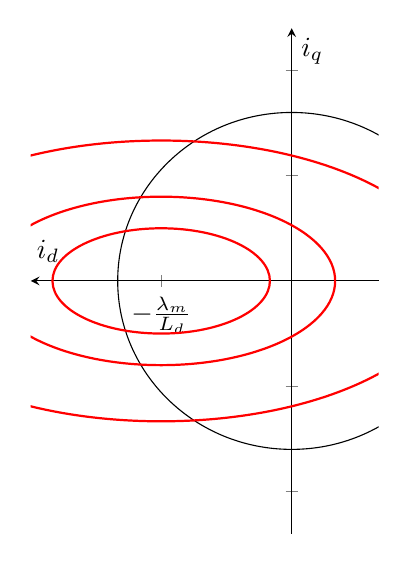
\begin{tikzpicture}
    \begin{axis}[
        axis lines=middle,
        width=6cm,
        height=8cm,
        xlabel={$i_d$},
        x label style={at={(axis description cs:0.05,0.6)},anchor=north},
        ylabel={$i_q$},
        %y label style={at={(axis description cs:0.95,0.05}},
        grid=none,
        xmin=-1.2,
        xmax=0.4,
        ymin=-1.2,
        ymax=1.2,
        no markers,
        x axis line style = {stealth-},
        xtick = {-0.6},
        xticklabels={$-\frac{\lambda_m}{L_d}$},  % Elimina las marcas en el eje x
        yticklabels=\empty,  % Elimina las marcas en el eje y
    ]
    
    
    \draw[black] (0,0) circle [radius=0.8];
    \draw[red, thick] (-0.6,0) ellipse (1.333333 and 0.66666666);
    \draw[red, thick] (-0.6,0) ellipse (0.8 and 0.4);
    \draw[red, thick] (-0.6,0) ellipse (0.5 and 0.25);

    \end{axis}
    \end{tikzpicture}
  \caption{Elipses de límite de voltaje con $I_{sc} \leq I_{s,max}$.}
\end{figure}




%% HASTA AQUI TRACUCCION POCHA DE LA WIKI

\section{Control del PMSM en el espacio d-q}
\subsection{Trayectorias de control}

Después de conocer los límites de la máquina, se pueden establecer criterios para decidir cuánto \(i_d\) y \(i_q\) (o \(I_s\) y \(\gamma\)) se deben aplicar al PMSM para que se comporte mecánicamente como se desee. El conjunto de puntos de trabajo que definen un comportamiento se llama trayectoria y existen una multitud de ellas. Por ejemplo, se puede desear que el motor produzca la mayor cantidad de par posible con la mínima corriente. Pero también se podría querer que tenga un cierto factor de potencia o que mantenga el par constante subiendo la velocidad, etc.

En un monoplaza de Formula Student, se desea que la salida de par esté perfectamente controlada y conocida para que el algoritmo de dinámica vehicular pueda estimar correctamente las fuerzas en los neumáticos. También es deseable que el motor pueda girar más rápido cuando no se requiere más par, ya que no es necesaria mucha tracción a altas velocidades del vehículo. Además, es necesario que sea eficiente para aprovechar mejor la energía de la batería. Con estos requisitos en mente, se estudian 4 trayectorias de control adecuadas para esta aplicación.

\subsubsection{MTPA (Máximo Par por Amperio)}

La trayectoria de control más utilizada es el MTPA, o Máximo Par por Amperio. Como su nombre indica, minimiza la corriente para entregar un par determinado. La condición que se debe cumplir es:

\begin{equation}
	\frac{\partial T_{em}}{\partial \gamma} = 0
\end{equation}


La expresión analítica se desarrolla como:

\begin{equation}
	T_{em} = \frac{3}{2}pp\cdot((L_d - L_q)\cdot I_s^2 \cdot \sin(\gamma)\cos(\gamma) + \lambda_m\cdot I_s\cdot \sin(\gamma))
\end{equation}


\begin{equation}
\frac{\partial T_{em}}{\partial \gamma} = \frac{\partial}{\partial \gamma} \frac{3}{2}pp\cdot(I_s^2 \cos(\gamma)\sin(\gamma)\cdot((L_d - L_q) + \lambda_m I_s \sin(\gamma)) = 0
\end{equation}

\begin{equation}
I_{s,\text{MTPA}} = -\frac{\lambda_m \cos(\gamma)}{(2\cdot\cos(\gamma)^2 - 1)\cdot(L_d-L_q)}
\end{equation}

Para la aplicación de esta trayectoria en el control se busca el ángulo como función de la corriente, y para ello se debe despejar \(\gamma_{MTPA}\) de la expresión.

\begin{equation}
\gamma_{\text{MTPA}} = \frac{\pi}{2} + \arcsin(\frac{\lambda_m \pm \sqrt{8(L_d-L_q)^2 \cdot I_s^2 + \lambda_m^2}}{4\cdot I_s(L_d-L_q)})
\end{equation}

El resultado de graficar esta expresión sobre el plano \((i_d, i_q)\) deja a la vista que el módulo de corriente es mínimo para cada hipérbola de par.


\begin{figure}[!ht]
  \centering
    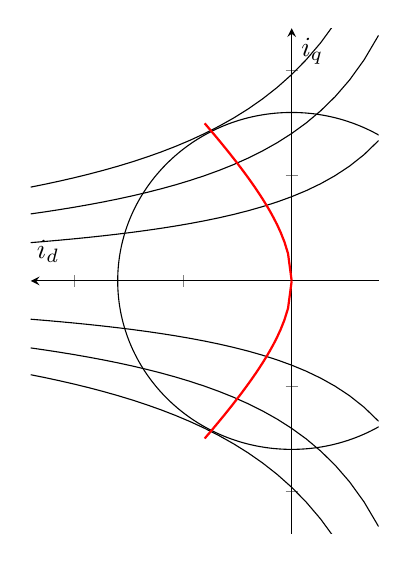
\begin{tikzpicture}
    \begin{axis}[
        axis lines=middle,
        width=6cm,
        height=8cm,
        xlabel={$i_d$},
        x label style={at={(axis description cs:0.05,0.6)},anchor=north},
        ylabel={$i_q$},
        %y label style={at={(axis description cs:0.95,0.05}},
        grid=none,
        xmin=-1.2,
        xmax=0.4,
        ymin=-1.2,
        ymax=1.2,
        no markers,
        x axis line style = {stealth-},
        xticklabels=\empty,  % Elimina las marcas en el eje x
        yticklabels=\empty,  % Elimina las marcas en el eje y
    ]
    
    \draw[black] (0,0) circle [radius=0.8];
    \addplot[black, domain=-1.2:0.4] {4*0.4/(3*2*((2/3)+(2/3)/1*(1-2)*x))};
    \addplot[black, domain=-1.2:0.4] {4*0.7/(3*2*((2/3)+(2/3)/1*(1-2)*x))};
    \addplot[black, domain=-1.2:0.4] {4*0.98/(3*2*((2/3)+(2/3)/1*(1-2)*x))};
    
    \addplot[black, domain=-1.2:0.4] {-4*0.4/(3*2*((2/3)+(2/3)/1*(1-2)*x))};
    \addplot[black, domain=-1.2:0.4] {-4*0.7/(3*2*((2/3)+(2/3)/1*(1-2)*x))};
    \addplot[black, domain=-1.2:0.4] {-4*0.98/(3*2*((2/3)+(2/3)/1*(1-2)*x))};
    
    \addplot[red, thick, domain=-0.4:0] {sqrt(((2/3)*x+(2/3)*(1-2)*x^2)/((2/3)*(1-2))))};
    \addplot[red, thick, domain=-0.4:0] {-sqrt(((2/3)*x+(2/3)*(1-2)*x^2)/((2/3)*(1-2))))};


    \end{axis}
    \end{tikzpicture}
  \caption{Trayectoria MTPA.}
\end{figure}


\subsubsection{CTC (Curva de Torque Constante)}

Como se puede observar, las hipérbolas de torque definen una trayectoria la cual permite mantener un par constante. Recordando las elipses de tensión, para un mismo valor de $V_s$ las elipses se contraen hacia el foco a medida que la velocidad aumenta. Esto significa que siguiendo la curva de torque constante de derecha a izquierda se puede mantener el par aumentando la velocidad. Usando la expresión del torque se puede obtener directamente:
\begin{equation}
	T_{em} = \frac{3}{2}pp\cdot((L_d - L_q)\cdot I_s^2 \cdot \sin(\gamma)\cos(\gamma) + \lambda_m\cdot I_s\cdot \sin(\gamma))
\end{equation}

\begin{equation}
I_{s,\text{CTC}} = \frac{\lambda_m}{L_d} \cdot \frac{\sqrt{\sin(\gamma)^2+\frac{2\cdot\frac{L_d-L_q}{L_d}\cdot\sin(2\gamma)\cdot T_{em}\cdot2 L_d}{3\cdot pp \cdot \lambda_m^2}}-\sin(\gamma)}{\sin(2\gamma)\cdot(\frac{L_d-L_q}{L_d})}
\end{equation}



\begin{figure}[!ht]
  \centering
    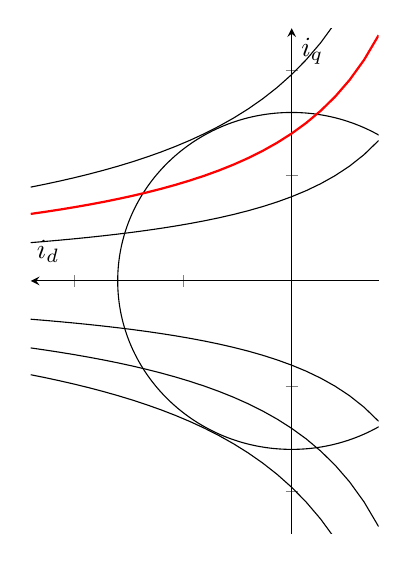
\begin{tikzpicture}
    \begin{axis}[
        axis lines=middle,
        width=6cm,
        height=8cm,
        xlabel={$i_d$},
        x label style={at={(axis description cs:0.05,0.6)},anchor=north},
        ylabel={$i_q$},
        %y label style={at={(axis description cs:0.95,0.05}},
        grid=none,
        xmin=-1.2,
        xmax=0.4,
        ymin=-1.2,
        ymax=1.2,
        no markers,
        x axis line style = {stealth-},
        xticklabels=\empty,  % Elimina las marcas en el eje x
        yticklabels=\empty,  % Elimina las marcas en el eje y
    ]
    
    \draw[black] (0,0) circle [radius=0.8];
    \addplot[black, domain=-1.2:0.4] {4*0.4/(3*2*((2/3)+(2/3)/1*(1-2)*x))};
    \addplot[red, thick, domain=-1.2:0.4] {4*0.7/(3*2*((2/3)+(2/3)/1*(1-2)*x))};
    \addplot[black, domain=-1.2:0.4] {4*0.98/(3*2*((2/3)+(2/3)/1*(1-2)*x))};
    
    \addplot[black, domain=-1.2:0.4] {-4*0.4/(3*2*((2/3)+(2/3)/1*(1-2)*x))};
    \addplot[black, domain=-1.2:0.4] {-4*0.7/(3*2*((2/3)+(2/3)/1*(1-2)*x))};
    \addplot[black, domain=-1.2:0.4] {-4*0.98/(3*2*((2/3)+(2/3)/1*(1-2)*x))};
    
    \end{axis}
    \end{tikzpicture}
  \caption{Trayectoria CTC.}
\end{figure}


\subsubsection{MTPV (Máximo Par por Voltio)}

Existe una trayectoria que permite maximizar el par entregado por el motor en rangos de velocidad muy altos donde el límite es la tensión que puede sintetizar la controladora. La condición que se debe cumplir es:

\begin{equation}
\frac{\partial T_{em}}{\partial \delta} = 0
\end{equation}

Donde $\delta$ es el ángulo del vector de tensión $V_s$. La expresión analítica se desarrolla como:

\begin{equation}
T_{em} = \frac{3}{2}pp\cdot((L_d - L_q) i_q i_d + \lambda_m i_q)
\end{equation}

Se neglige la caída de tensión resistiva del estator. 
\begin{equation}
i_d = \frac{v_q}{\omega_e \cdot L_d} - \frac{\lambda_m}{L_d}; i_q = -\frac{v_d}{\omega_e \cdot L_q}
\end{equation}

\begin{equation}
T_{em} = \frac{3}{2}pp\cdot\left((L_d - L_q) (-\frac{v_d}{\omega_e \cdot L_q}) (\frac{v_q}{\omega_e \cdot L_d} - \frac{\lambda_m}{L_d}) + \lambda_m (-\frac{v_d}{\omega_e \cdot L_q})\right)
\end{equation}

\begin{equation}
T_{em} = \frac{3}{2}pp\cdot\left((L_d - L_q) (-\frac{V_s \cdot \cos(\delta)}{\omega_e \cdot L_q}) (\frac{V_s \cdot \sin(\delta)}{\omega_e \cdot L_d} - \frac{\lambda_m}{L_d}) + \lambda_m (-\frac{V_s \cdot \cos(\delta)}{\omega_e \cdot L_q})\right)
\end{equation}

\begin{equation}
\begin{split}
\frac{\partial T_{em}}{\partial \delta} = \frac{3}{2}pp\cdot (
(L_d - L_q) \cdot (\frac{V_s \cdot \sin(\delta)}{\omega_e \cdot L_q}) \cdot (\frac{V_s \cdot \sin(\delta)}{\omega_e \cdot L_d} - \frac{\lambda_m}{L_d})\\
-\left(\frac{V_s \cdot \cos(\delta)}{\omega_e}\right)^2 \cdot \frac{L_d - L_q}{L_d\cdot L_q}\\ 
-\frac{\lambda_m \cdot V_s \cdot \sin(\delta)}{L_q \cdot \omega_e} ) = 0
\end{split}
\end{equation}


\begin{equation}
\begin{split}
I_{s,MTPV} = \frac{\lambda_m}{L_d} ( \frac{-(2 - \frac{L_q}{L_d}) \cos(\gamma)}{2(1 - \frac{L_q}{L_d})(1 + (\frac{L_q}{L_d})^2) \cos(\gamma)^2 - 2(1 - \frac{L_q}{L_d}) (\frac{L_q}{L_d})^2}\\
-\frac{\sqrt{(2 - \frac{L_q}{L_d})^2 \cos(\gamma)^2 - 4(1 - \frac{L_q}{L_d})(1 + (\frac{L_q}{L_d})^2) \cos(\gamma)^2 - 4(1 - \frac{L_q}{L_d}) (\frac{L_q}{L_d})^2}}{2(1 - \frac{L_q}{L_d})(1 + (\frac{L_q}{L_d})^2) \cos(\gamma)^2 - 2(1 - \frac{L_q}{L_d}) (\frac{L_q}{L_d})^2} )
\end{split}
\end{equation}




Cabe destacar que esta trayectoria solamente se puede ejecutar si se cumple la condición de que $I_{sc} \leq I_{s,max}$.


\begin{figure}[!ht]
  \centering
    \begin{tikzpicture}
    \begin{axis}[
        axis lines=middle,
        width=6cm,
        height=8cm,
        xlabel={$i_d$},
        x label style={at={(axis description cs:0.05,0.6)},anchor=north},
        ylabel={$i_q$},
        %y label style={at={(axis description cs:0.95,0.05}},
        grid=none,
        xmin=-1.2,
        xmax=0.4,
        ymin=-1.2,
        ymax=1.2,
        no markers,
        x axis line style = {stealth-},
        xtick = {-0.6},
        xticklabels={$-\frac{\lambda_m}{L_d}$},  % Elimina las marcas en el eje x
        yticklabels=\empty,  % Elimina las marcas en el eje y
    ]
    
    
    \draw[black] (0,0) circle [radius=0.8];
    \addplot[red, thick, domain=-0.77:-0.6] {0.5*sqrt(4*(1.111111)^2*(x^2-x*0)+(1.111111)^2*0^2-2.22222222^2*0.6^2)/2.22222222};


    \end{axis}
    \end{tikzpicture}
  \caption{Trayectoria MTPV.}
\end{figure}



\subsubsection{CVL (Límites de Corriente y Voltaje)}

Por último, se presentan los límites eléctricos del motor y del convertidor. El límite de corriente consiste simplemente en saturar la magnitud de la corriente de manera que no sobrepase el valor máximo establecido. La trayectoria sería sencillamente seguir el círculo de corriente anteriormente presentado (CLC), con la siguiente expresión:

\[
I_{s,\text{CLC}} = I_{s,\text{max}} , \forall \gamma \in [0,2\pi]
\]



\begin{figure}[!ht]
  \centering
    \begin{tikzpicture}
    \begin{axis}[
        axis lines=middle,
        width=6cm,
        height=8cm,
        xlabel={$i_d$},
        x label style={at={(axis description cs:0.05,0.6)},anchor=north},
        ylabel={$i_q$},
        %y label style={at={(axis description cs:0.95,0.05}},
        grid=none,
        xmin=-1.2,
        xmax=0.4,
        ymin=-1.2,
        ymax=1.2,
        no markers,
        x axis line style = {stealth-},
        xticklabels=\empty,  % Elimina las marcas en el eje x
        yticklabels=\empty,  % Elimina las marcas en el eje y
    ]
    
    % Límite de corriente Is_max
    \draw[red, thick] (0,0) circle [radius=0.8];

    \end{axis}
    \end{tikzpicture}
  \caption{Trayectoria CLC.}
\end{figure}


El límite de tensión del motor en realidad se puede entender como la velocidad máxima a la que se puede llegar con una determinada tensión. Por ello, se usa la expresión de las elipses de tensión (VLE):

\begin{equation}
1 \geq \frac{\left(\frac{\lambda_m}{L_d}+I_s \cdot \cos(\gamma)\right)^2}{\left(\frac{\frac{V_{DC}}{\sqrt{3}}}{\omega_e}\right)^2}+\frac{(L_q+I_s \cdot \sin(\gamma))^2}{\left(\frac{\frac{V_{DC}}{\sqrt{3}}}{\omega_e}\right)^2}
\end{equation}

Igual que para el resto de trayectorias, se debe obtener una expresión de la elipse en función de $I_s$ y $\gamma$. Ya que no es trivial despejar estas variables de la expresión anterior, se manipula usando la ecuación polar de la elipse desplazada del origen:
\begin{equation}
\rho(\theta) = \frac{b^2 x \cos (\theta ) + a^2 y \sin (\theta )\pm a b \sqrt{\left(a^2-x^2\right) \sin ^2(\theta )+\left(b^2-y^2\right) \cos ^2(\theta )+2 x y \sin (\theta ) \cos (\theta )}}{a^2 \sin ^2(\theta )+b^2 \cos ^2(\theta )}
\end{equation}

Dado que estas elipses tan solo están desplazadas en el eje $x$, se pueden eliminar todos los términos referentes al desplazamiento en $y$.
\begin{equation}
\rho(\theta) = \frac{b^2 x \cos (\theta ) \pm a b \sqrt{\left(a^2-x^2\right) \sin ^2(\theta )+\left(b^2\right) \cos ^2(\theta )}}{a^2 \sin ^2(\theta )+b^2 \cos ^2(\theta )}
\end{equation}

Sustituyendo por los términos conocidos:

\begin{equation}
I_{s,\text{VLE}} = \frac{\left(\frac{V_s}{L_q\cdot \omega_e}\right)^2 \left(-\frac{\lambda_m}{L_d}\right) \cos (\gamma) \pm \frac{V_s}{L_d\cdot \omega_e} \frac{V_s}{L_q\cdot \omega_e} \sqrt{\left(\frac{V_s}{L_d\cdot \omega_e}\right)^2- \left(-\frac{\lambda_m}{L_d}\right)^2 \sin^2(\gamma) + \left(\frac{V_s}{L_q\cdot \omega_e}\right)^2 \cos^2(\gamma)}}{\left(\frac{V_s}{L_d\cdot \omega_e}\right)^2 \sin^2(\gamma) + \left(\frac{V_s}{L_q\cdot \omega_e}\right)^2 \cos^2(\gamma)}
\end{equation}


\begin{figure}[!ht]
  \centering
    \begin{tikzpicture}
    \begin{axis}[
        axis lines=middle,
        width=6cm,
        height=8cm,
        xlabel={$i_d$},
        x label style={at={(axis description cs:0.05,0.6)},anchor=north},
        ylabel={$i_q$},
        %y label style={at={(axis description cs:0.95,0.05}},
        grid=none,
        xmin=-1.2,
        xmax=0.4,
        ymin=-1.2,
        ymax=1.2,
        no markers,
        x axis line style = {stealth-},
        xtick = {-1},
        xticklabels={$-\frac{\lambda_m}{L_d}$},  % Elimina las marcas en el eje x
        yticklabels=\empty,  % Elimina las marcas en el eje y
    ]
    
    
    \draw[black] (0,0) circle [radius=0.8];

    \draw[red, thick] (-1,0) ellipse (0.5 and 0.25);


    \end{axis}
    \end{tikzpicture}
  \caption{Trayectoria VLE.}
\end{figure}



Además, el inversor es capaz de sintetizar un máximo de $V_s = \frac{V_{DC}}{\sqrt{3}}$ utilizando SVPWM, por lo tanto, se debe saturar la consigna de tensión a ese valor. Adicionalmente, por seguridad, se multiplica por un factor de seguridad $K_{FW}$ menor a 1.

\begin{equation}
	V_{s,\text{max}} \leq \frac{V_{DC}}{\sqrt{3}}\cdot K_{FW}
\end{equation}

\subsection{Diseño y simulación del control}

En esta sección, se aborda la implementación del modelo matemático del PMSM en un entorno de simulación. Además, se detallan los pasos cruciales en el diseño del control, destacando la implementación del lazo de control de corriente, el modelo promediado y conmutado del inversor, o la integración de las trayectorias y la estrategia de debilitamiento de campo. Disponer de un modelo de simulación completo permite ganar mucha comprensión sobre el sistema estudiado, pero por el coste computacional suele ser inviable juntar muchos sistemas en una misma simulación.

\subsubsection{EMR (Representación macroscópica energética)}
En primer lugar, se tratará de crear un modelo que permita simular la dinámica electromecánica del PMSM, así como el entorno mecánico en el que se encuentra (vehículo eléctrico) e integrar el control vectorial. Para ello se usará un estándar para modelizar sistemas de potencia, la representación macroscópica energética o EMR por sus siglas en inglés. El concepto se basa en agrupar o dividir las diferentes etapas en las que la potencia se transforma, utilizando el principio de acción-reacción\textit{ y el principio causal (la causa del efecto causa-efecto es que el efecto causa-efecto es a su vez causa y efecto)}. 

En primer lugar se modeliza la planta eléctrica del PMSM. Se utiliza el modelo con el marco de referencia rotativo $d-q$ por su sencillez. Para ello se implementan las diferentes ecuaciones del motor y se implementan en bloques separados siguiendo el estándar de la EMR.

\begin{figure}[!ht]
    \centering
    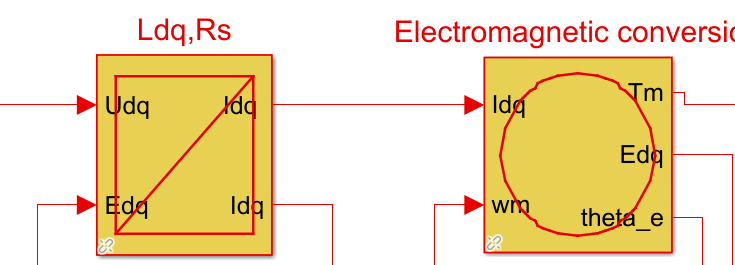
\includegraphics[width=0.7\linewidth]{fig/motorEMR1.png}
    \caption{Bloques que representan el PMSM.}
\end{figure}

\begin{figure}[!ht]
    \centering
    \begin{subfigure}{0.52\linewidth}
        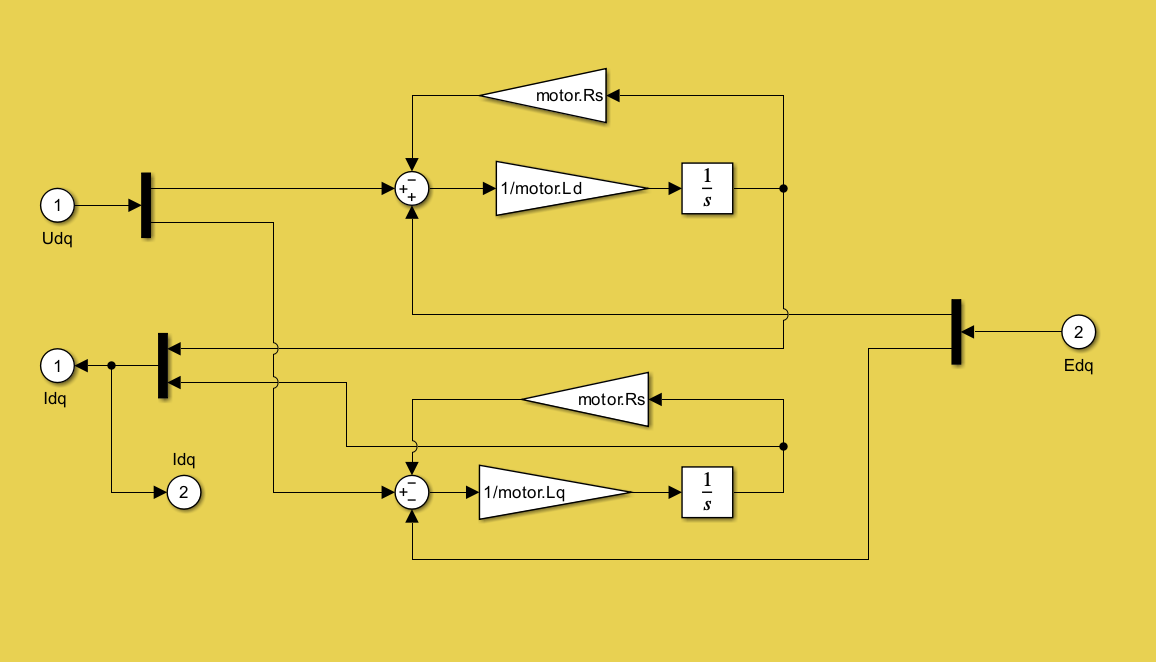
\includegraphics[width=\linewidth]{fig/motorEMR2.png}
        \caption{Circuito eléctrico.}
    \end{subfigure}
    \begin{subfigure}{0.4\linewidth}
        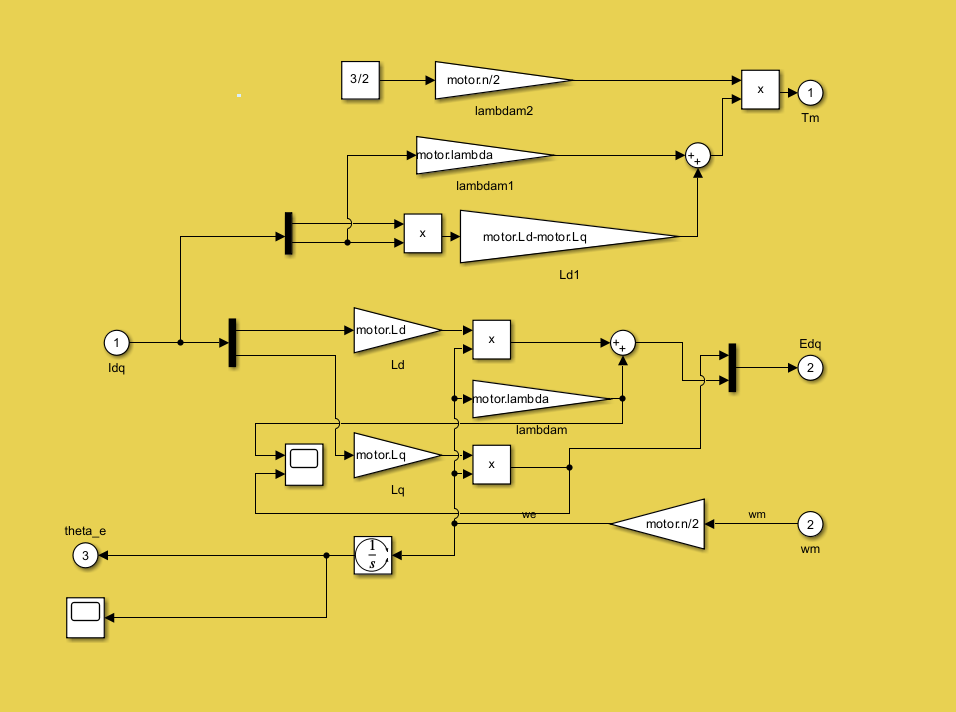
\includegraphics[width=\linewidth]{fig/motorEMR3.png}
        \caption{Conversión electromecánica}
    \end{subfigure}
    \caption{Detalle de los bloques del PMSM}
\end{figure}

También se modela la planta mecánica del motor, así como la transmisión de la potencia mecánica a las ruedas y al vehículo.

\begin{figure}[!ht]
    \centering
    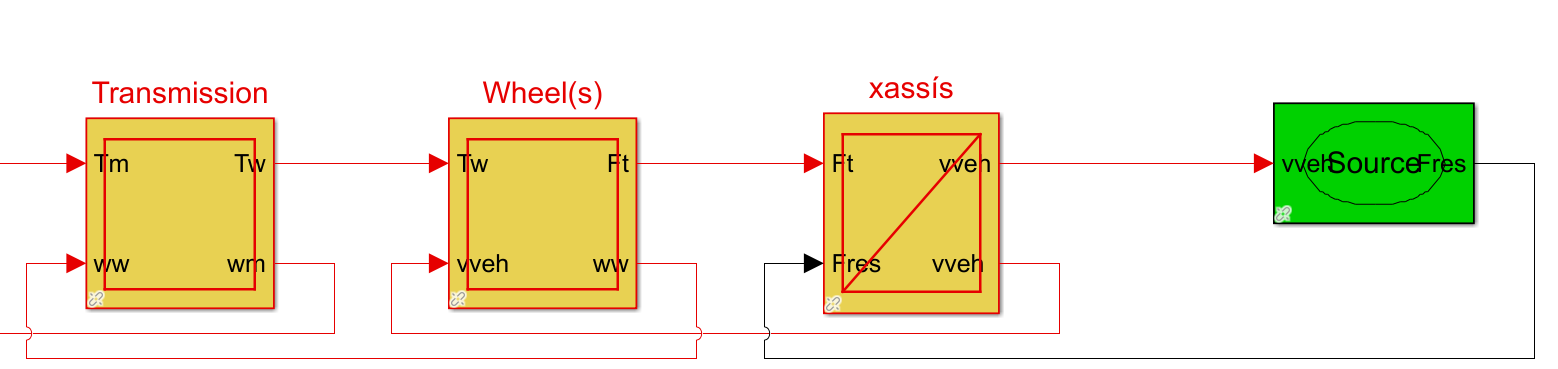
\includegraphics[width=0.95\linewidth]{fig/carEMR.png}
    \caption{Planta mecánica.}
\end{figure}

\subsubsection{Lazos de corriente y modelo promediado del inversor}

Como se ha visto hasta ahora, es práctico utilizar la corriente para controlar el motor. Por ello, se implementa un lazo de corriente utilizando controladores PI para el eje $d$ y para el eje $q$ por separado. Como el inversor se utiliza como fuente de tensión, la salida de estos PI es la consigna de tensión. Dado que el motor genera una BEMF (fuerza contra-electromotriz), se añade como \textit{feed-forward} a los controladores. La salida del controlador no se satura directamente, sino que se implementa una saturación posterior la cual se realimenta al controlador para usar una técnica de \textit{anti-windup}. Las constantes de los controladores se ajustan de la siguiente manera:

% PI de corriente, respuesta de segundo orden
\[
M_p = 15\% , t_s = T_s \cdot 20
\]

Donde $T_s$ es la inversa de la frecuencia de control.

\[
\xi = \sqrt{\frac{\log(M_p)^2}{\pi^2 + \log(M_p)^2}}
\]
\[
\omega_n = \frac{3}{\xi \cdot t_s}
\]
\[
Kp_{id} = 2 \cdot \xi \cdot \omega_n \cdot L_d - r_s
\]
\[
Ki_{id} = \omega_n^2 \cdot L_d
\]
\[
Kp_{iq} = 2 \cdot \xi \cdot \omega_n \cdot L_q - r_s
\]
\[
Ki_{iq} = \omega_n^2 \cdot L_q \quad
\]

\begin{figure}[!ht]
    \begin{subfigure}{0.2\linewidth}
        \centering
        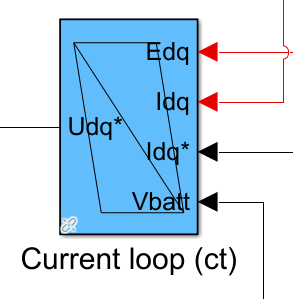
\includegraphics[width=\linewidth]{fig/PIEMR_out.png}
    \end{subfigure}
    \begin{subfigure}{0.75\linewidth}
        \centering
        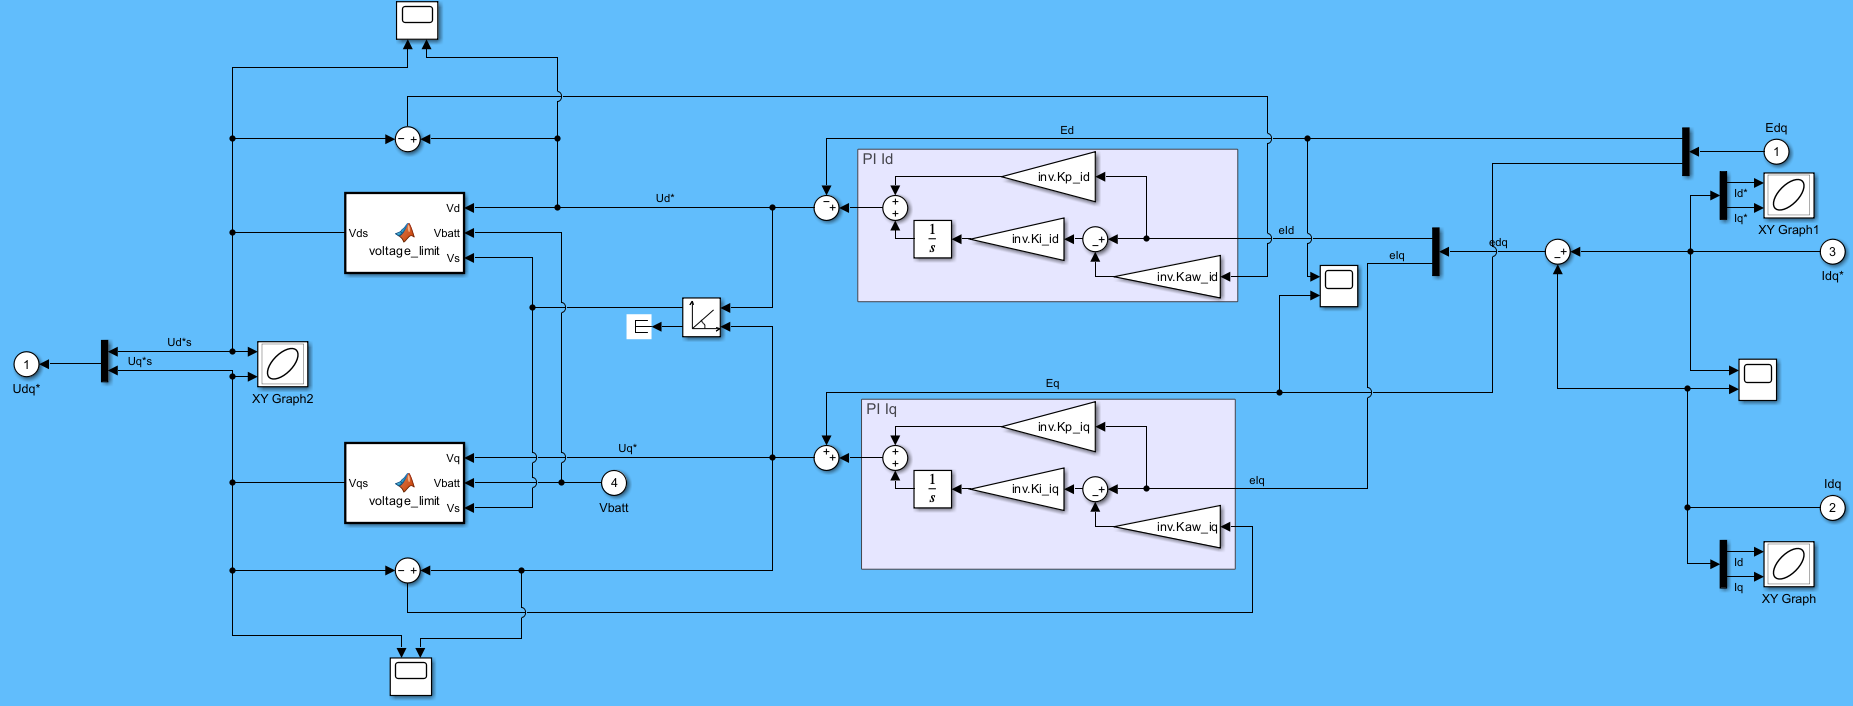
\includegraphics[width=\linewidth]{fig/PIEMR_in.png}
    \end{subfigure}
    \caption{Bloque de los lazos de corriente.}
\end{figure}

Para las simulaciones se han implementado los siguientes parámetros de motor, ya que aunque a fecha de redacción de este documento no está fabricado, se han estimado de manera que se cumplan los requisitos del motor.


\begin{tabular}{|p{2cm}||p{1cm}|p{1.5cm}|p{7cm}|}
 \hline
 \multicolumn{4}{|c|}{Parámetros del Motor} \\
 \hline
 Parámetro & Valor & Unidades & Descripción \\
 \hline
 pp & 3 & ad & Número de pares de polos \\
 $\lambda_m$ & 52.615 & mWb & Flujo magnético de los imanes permanentes \\
 $L_d$ & 1.887 & mH & Inductancia en el eje d \\
 $L_q$ & 2.831 & mH & Inductancia en el eje q \\
 $R_s$ & 150 & m$\Omega$ & Resistencia de fase del estator \\
 $\omega_{\text{m,max}}$ & 20000 & rpm & Velocidad angular máxima del motor \\
 $T_{\text{em,max}}$ & 26 & N·m & Par máximo del motor \\
 $V_{\text{bat}}$ & 540 & V & Voltaje de la batería DC \\
 $I_{\text{s,max}}$ & 108 & A & Corriente máxima en los ejes d-q \\
 \hline
\end{tabular}



\begin{figure}[!ht]
    \centering
    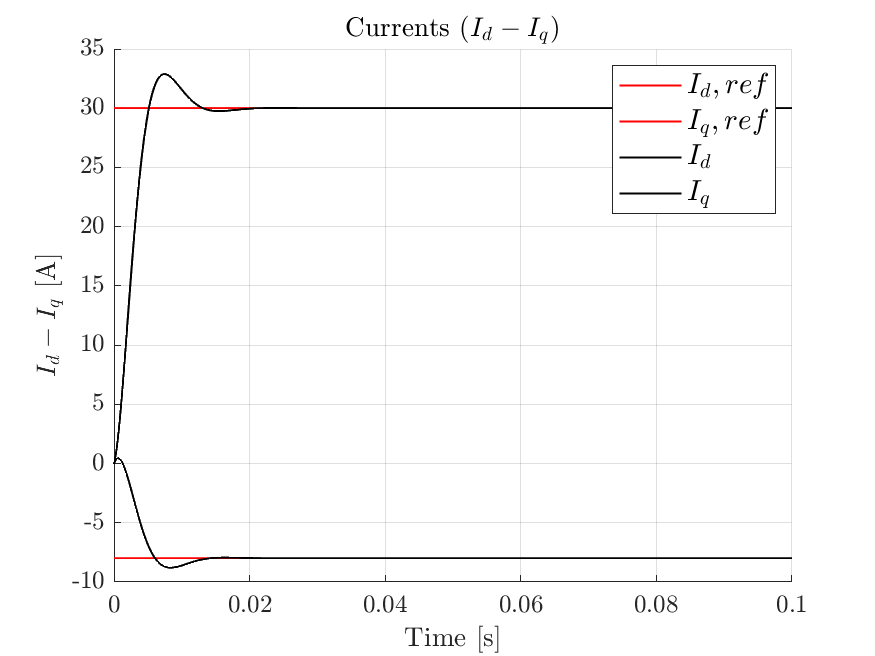
\includegraphics[width=0.75\linewidth]{fig/idiq_plot_PI.png}
    \caption{Simulación de los PIs de corriente, con una consigna de $(i_d, i_q) = (-8, 30) A$}
\end{figure}


Tras obtener las consignas de tensión, se modela el inversor VSI con SVPWM con un modelo promediado, es decir, sin llegar a generar una señal conmutada por PWM. Se usan relaciones básicas para convertir las magnitudes eléctricas del espacio $d-q$ a DC. Además se incorpora la fuente de energía del sistema, la batería, con un simple modelo RC.

\begin{figure}[!ht]
    \centering
    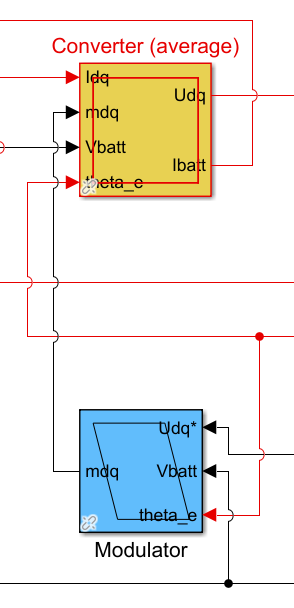
\includegraphics[width=0.25\linewidth]{fig/VSIEMR_out.png}
    \caption{Bloques que contienen el modelo promediado del VSI con SVPWM.}

\end{figure}

\begin{figure}[!ht]
    \centering
    \begin{subfigure}{0.45\linewidth}
        \centering
        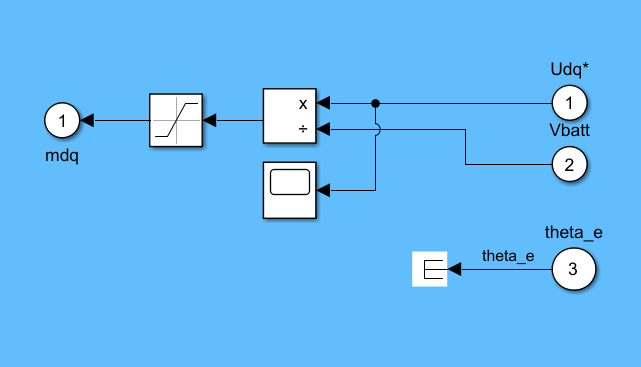
\includegraphics[width=\linewidth]{fig/VSIEMR_in1.png}
    \end{subfigure}
    \begin{subfigure}{0.45\linewidth}
        \centering
        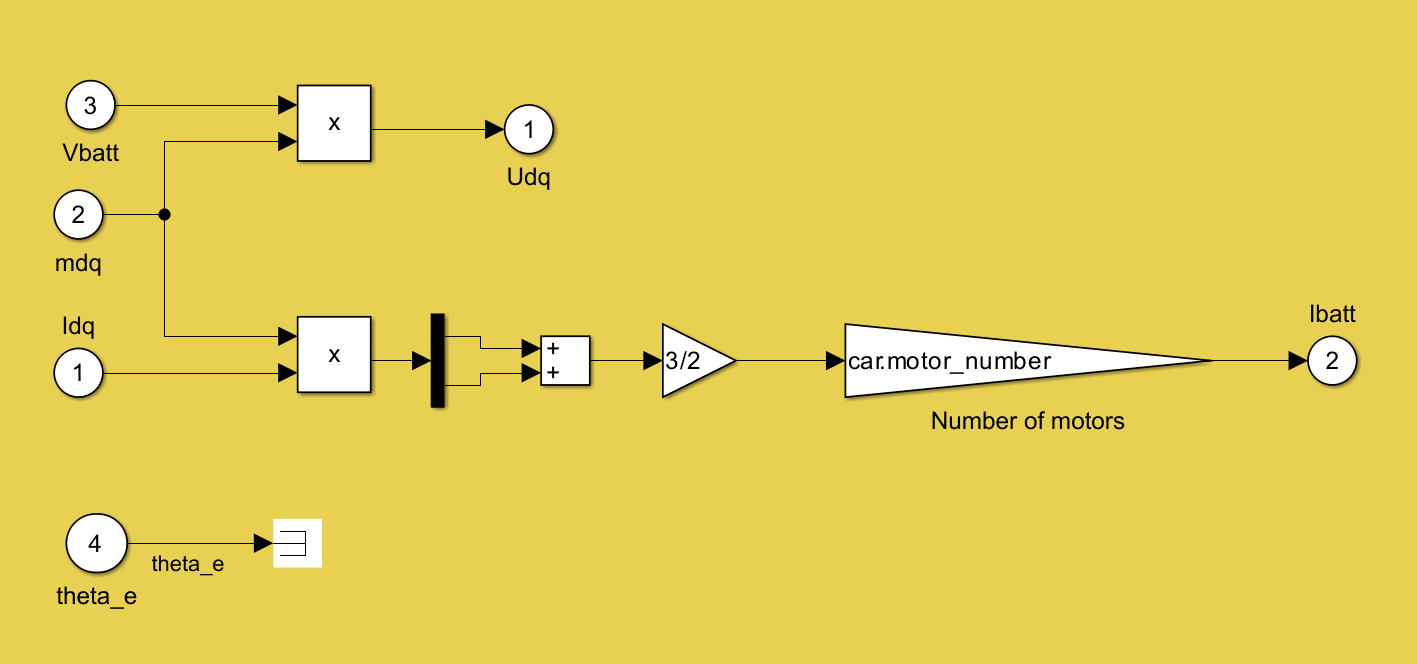
\includegraphics[width=\linewidth]{fig/VSIEMR_in2.png}
    \end{subfigure}
    \caption{Detalle de los bloques del VSI.}

\end{figure}

\subsubsection{Implementación de las trayectorias de control}

Con lo anteriormente desarrollado solamente se pueden consignar las corrientes $i_d$ e $i_q$ manualmente, pero el objetivo es consignar el par y que el propio control sea capaz de gestionar el debilitamiento de campo. Por ello, se implementan las ecuaciones presentadas en el apartado anterior en bloques de código. 

La estrategia es la siguiente: Se implementan las ecuaciones de las trayectorias cuya salida es una corriente (CLC, CTC, MTPV y VLE) y se selecciona la mínima, o en caso de estar en zona de debilitamiento de campo, la óptima, que no necesariamente es la mínima. En paralelo, se calcula el ángulo que correspondería a la trayectoria del MTPA, y se añade un control integral que aumenta el valor del ángulo controlando la tensión para poder entrar en el resto de trayectorias. Se trabaja con módulos de corriente siempre positivos, y ángulos comprendidos entre $\gamma \in [\frac{\pi}{2}, \pi]$. Para obtener par negativo, simplemente se multiplica el ángulo $\gamma$ por el signo de la consigna de par.

De entre aquellas ecuaciones cuya salida es la corriente $I_s$, se usa la que computa un valor más pequeño, limitando así el módulo. Además, se calcula el ángulo correspondiente a la trayectoria del MTPA, y se usa un integrador para modificar el ángulo y poder usar las trayectorias consideradas como debilitamiento de campo. Este integrador se encarga de que la consigna de ángulo no haga sobrepasar el límite de tensión establecido por el inversor. 

\begin{figure}[!ht]
    \centering
    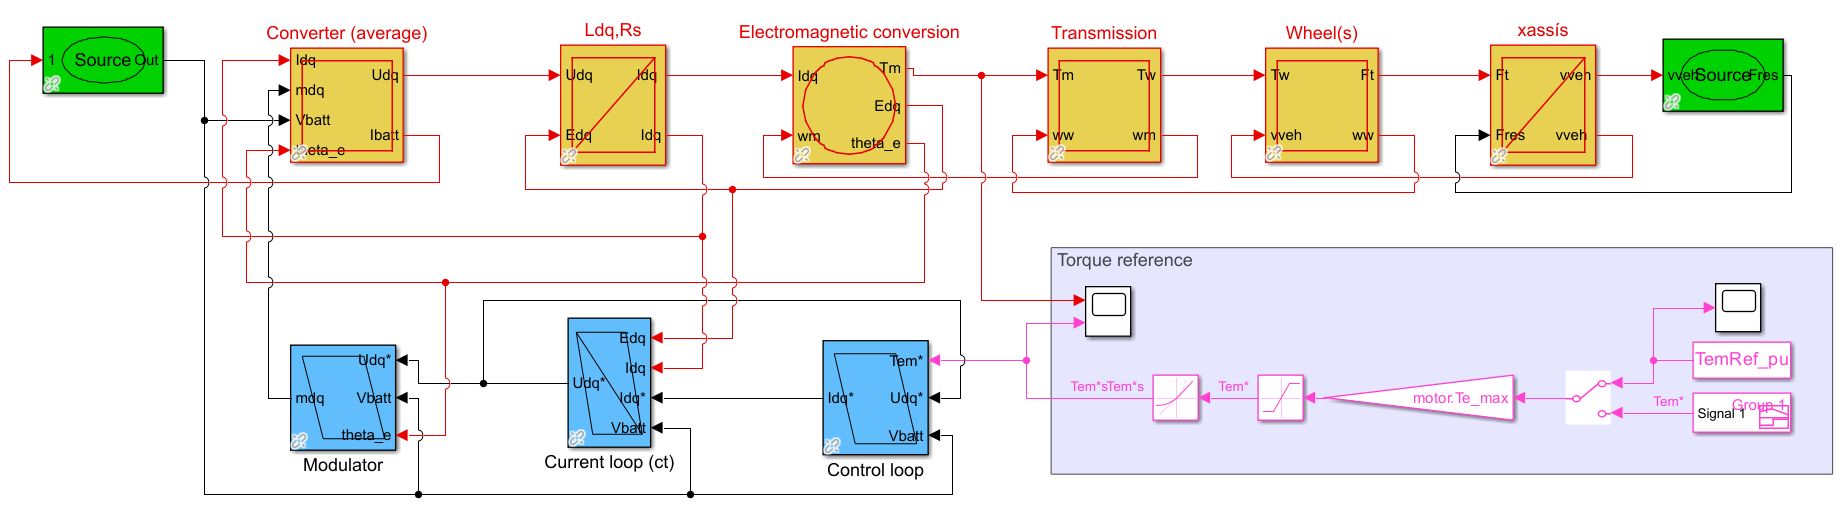
\includegraphics[width=1\linewidth]{fig/EMR_FULL.png}
    \caption{Modelo EMR completo.}
    
\end{figure}

\begin{figure}[!ht]
    \centering
    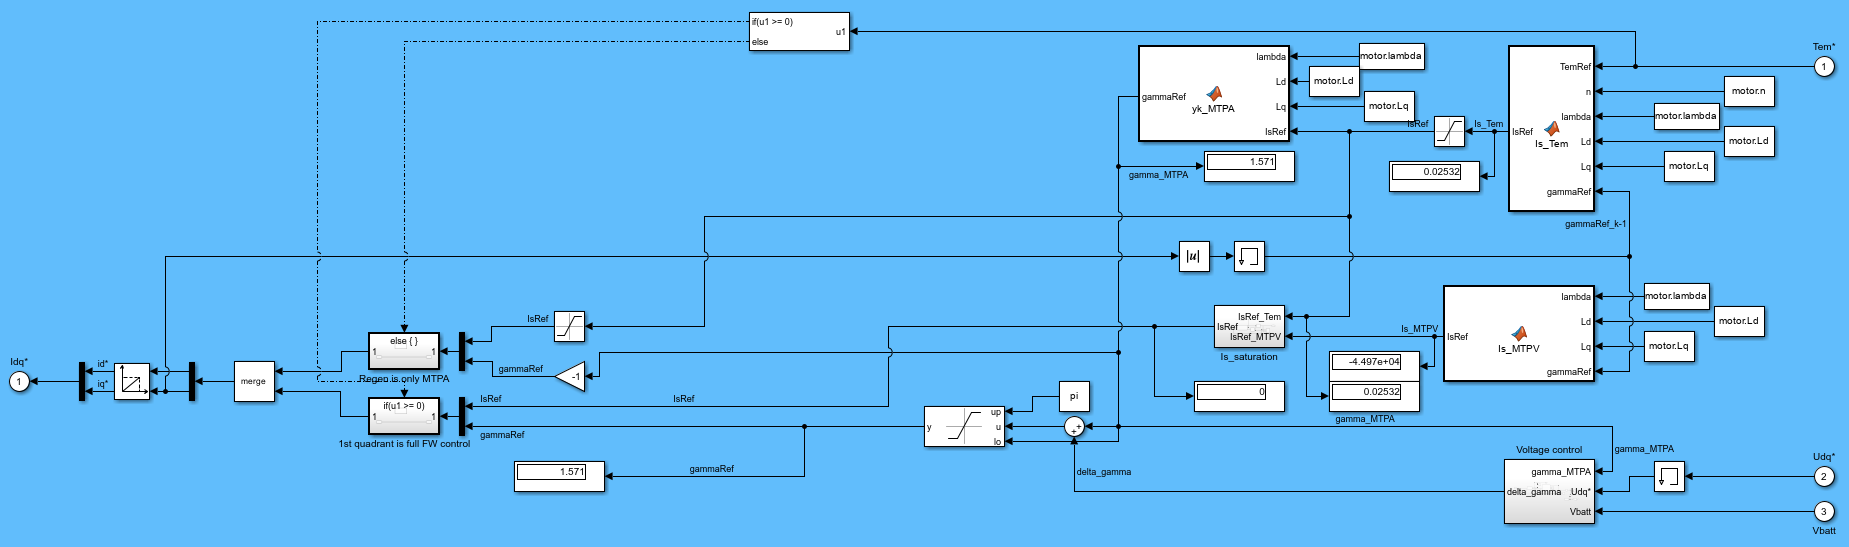
\includegraphics[width=1\linewidth]{fig/EMR_control.png}
    \caption{Detalle del bloque del lazo de control vectorial.}
    
\end{figure}

Para comprobar el funcionamiento y la estabilidad del control, se realiza una simulación en la que la consigna de par está extraída de un perfil de conducción real.

\begin{figure}[!ht]
    \centering

    \begin{subfigure}{0.4\textwidth}
        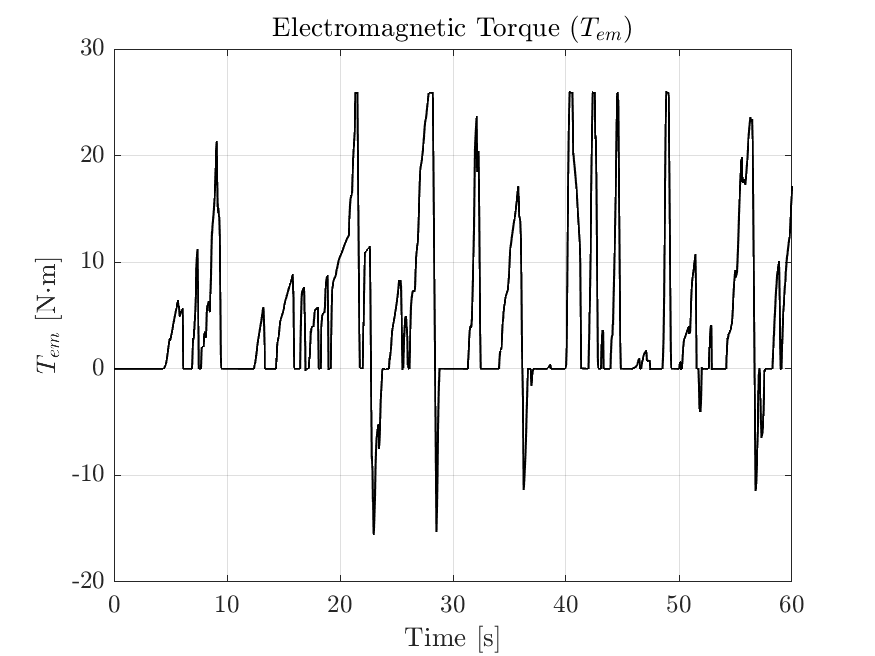
\includegraphics[width=\linewidth]{fig/Tem_plot.png}
        \caption{Torque electromagnético ($T_{em}$)}
    \end{subfigure}
    %
    \begin{subfigure}{0.4\textwidth}
        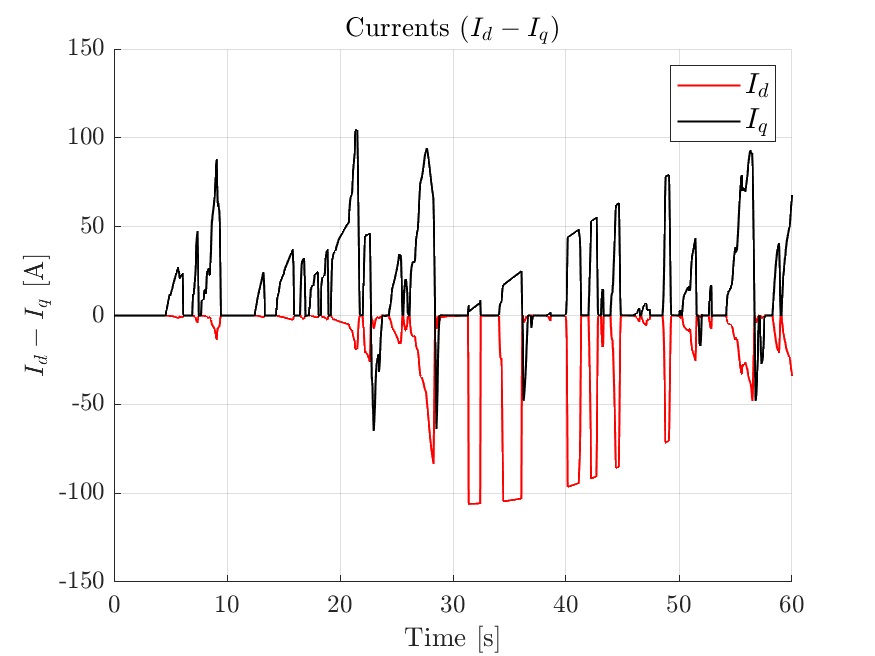
\includegraphics[width=\linewidth]{fig/idiq_plot.png}
        \caption{Corrientes ($I_{d} - I_{q}$)}
    \end{subfigure}

    \begin{subfigure}{0.4\textwidth}
        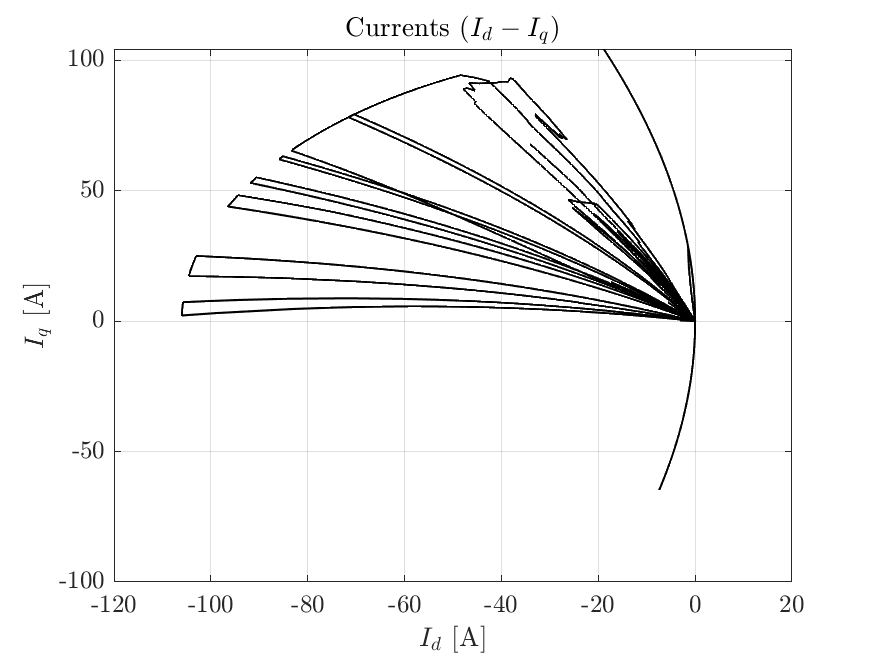
\includegraphics[width=\linewidth]{fig/id-iq_plot.png}
        \caption{Corriente ($I_{d}$) vs Corriente ($I_{q}$)}
    \end{subfigure}
    %
    \begin{subfigure}{0.4\textwidth}
        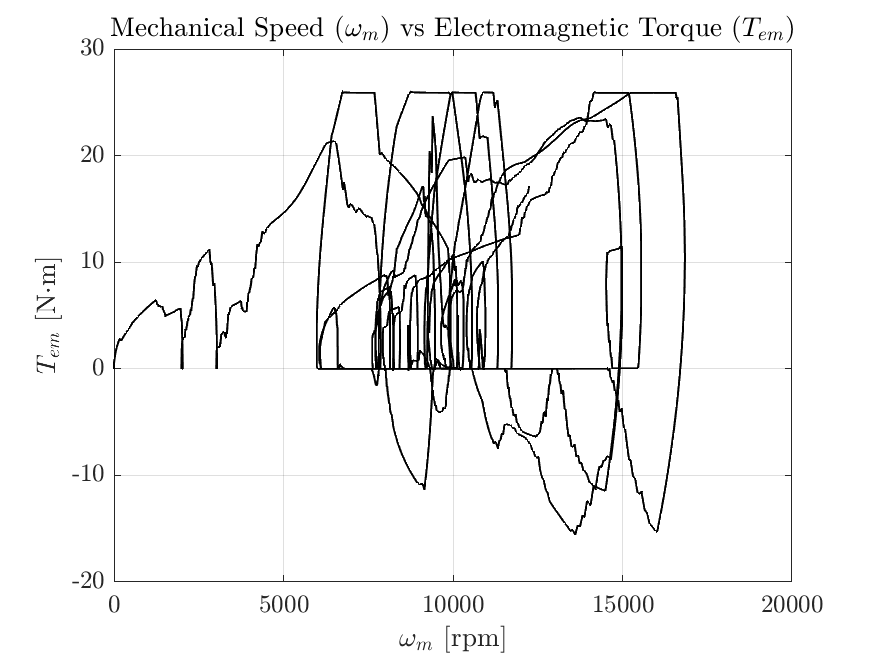
\includegraphics[width=\linewidth]{fig/wm_Tem_plot.png}
        \caption{Velocidad mecánica ($\omega_{m}$) vs Torque electromagnético ($T_{em}$)}
    \end{subfigure}

    \begin{subfigure}{0.4\textwidth}
        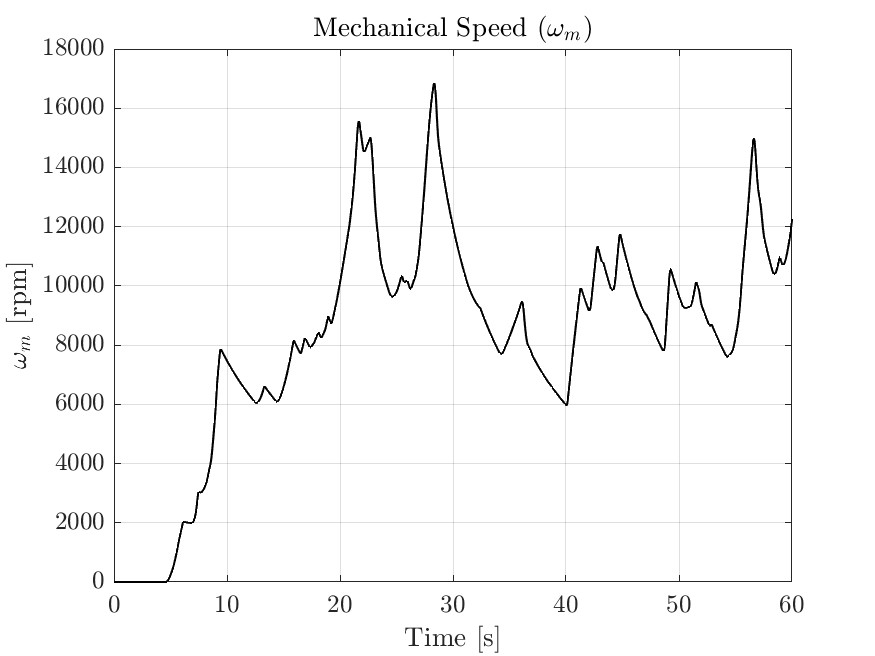
\includegraphics[width=\linewidth]{fig/wm_plot.png}
        \caption{Velocidad mecánica ($\omega_{m}$)}
    \end{subfigure}
    %
    \begin{subfigure}{0.4\textwidth}
        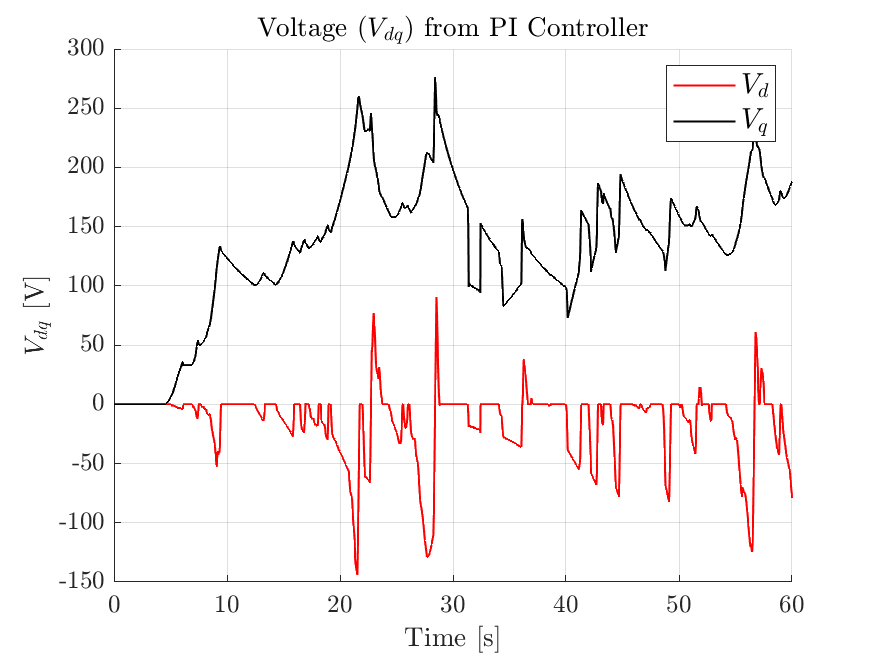
\includegraphics[width=\linewidth]{fig/vdvqPI_plot.png}
        \caption{Voltajes ($V_{d} - V_{q}$)}
    \end{subfigure}

    \caption{Resultados de la simulación.}
\end{figure}

Se puede observar que en esta simulación se ha limitado el comportamiento de la frenada regenerativa a la trayectoria del MTPA. En la implementación real se han explorado los límites para poder ofrecer una mejor respuesta del motor regenerando a altas velocidades.

\subsubsection{Modelo conmutado en PLECS}

Dado que el inversor realmente es una fuente conmutada, se debe modelar utilizando una herramienta que lo permita. Utilizando el modelo EMR generado en Simulink se ha implementado la conmutación, pero el tiempo de simulación es demasiado grande como para que sea una herramienta práctica para el desarrollo.

\begin{figure}[!ht]
    \centering
    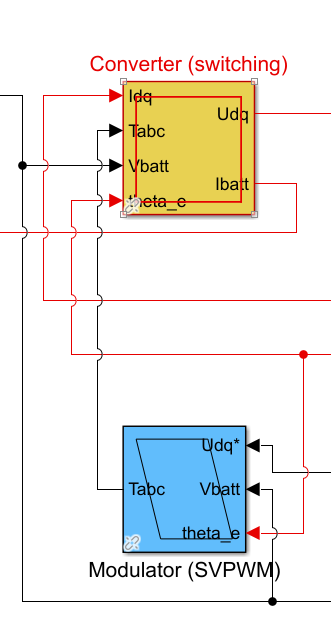
\includegraphics[width=0.25\linewidth]{fig/EMR_VSIsw_out.png}
    \caption{Bloques que contienen el modelo conmutado del VSI con SVPWM.}
    
\end{figure}

\begin{figure}[!ht]
    \centering

    \begin{subfigure}{0.75\linewidth}
        \centering
        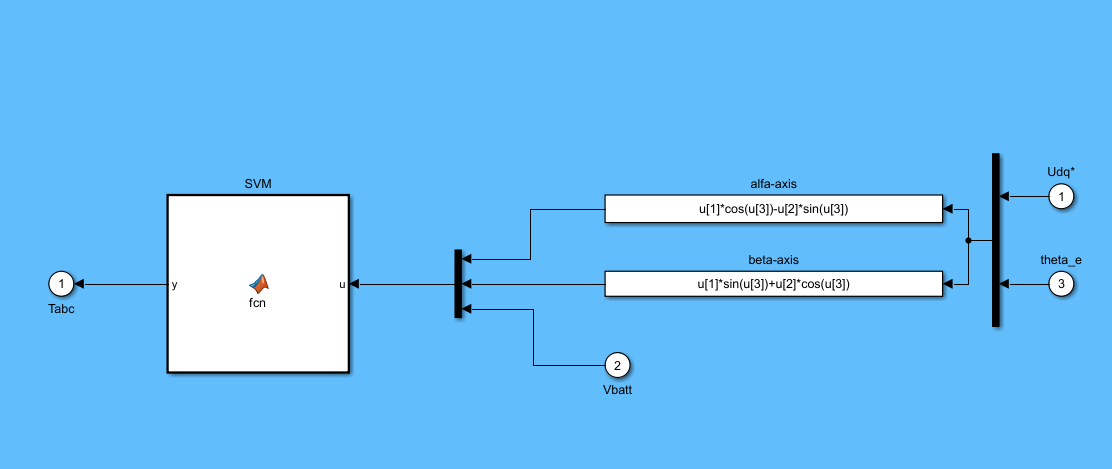
\includegraphics[width=\linewidth]{fig/EMR_VSIsw_in1.png}   
    \end{subfigure}
    \begin{subfigure}{0.75\linewidth}
        \centering
        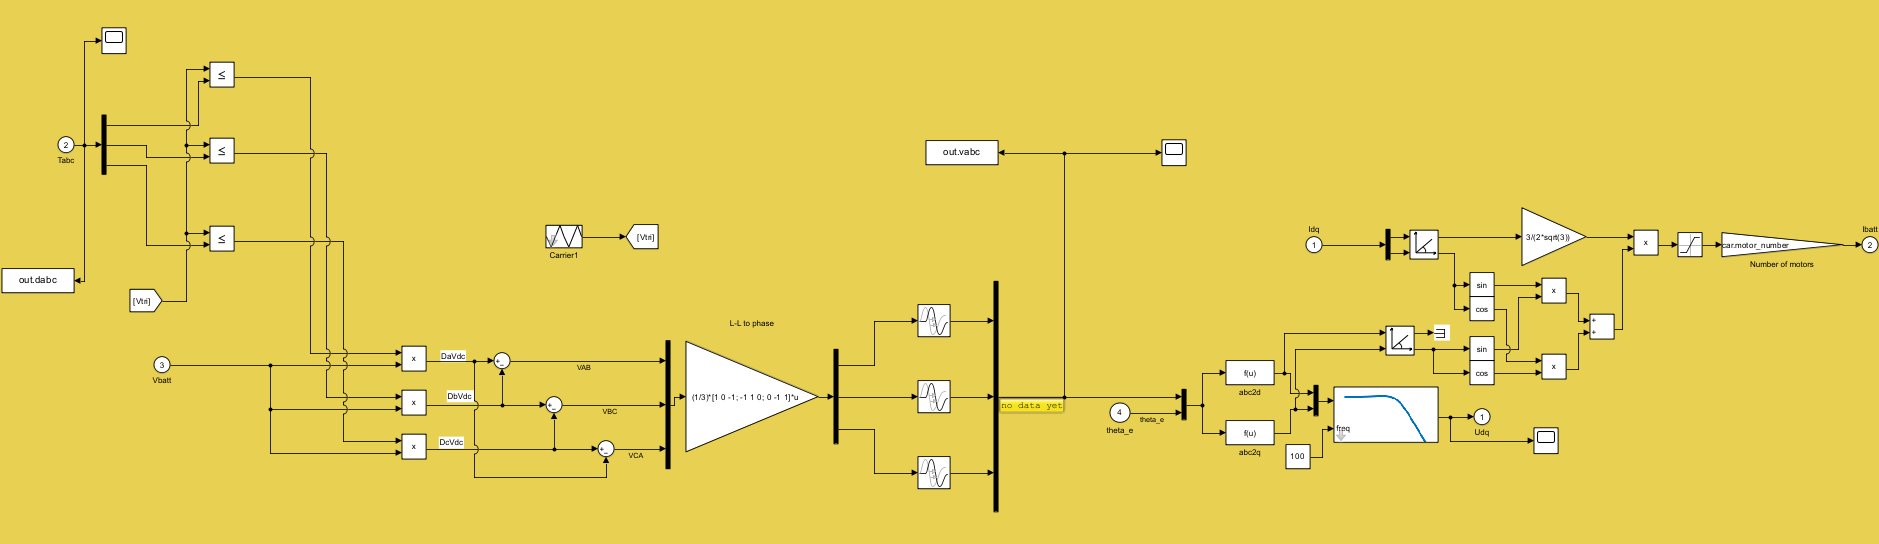
\includegraphics[width=\linewidth]{fig/EMR_VSIsw_in2.png}
    \end{subfigure}
    \caption{Detalle de los bloques del VSI conmutado.}

\end{figure}


\begin{figure}[!ht]
    \centering
    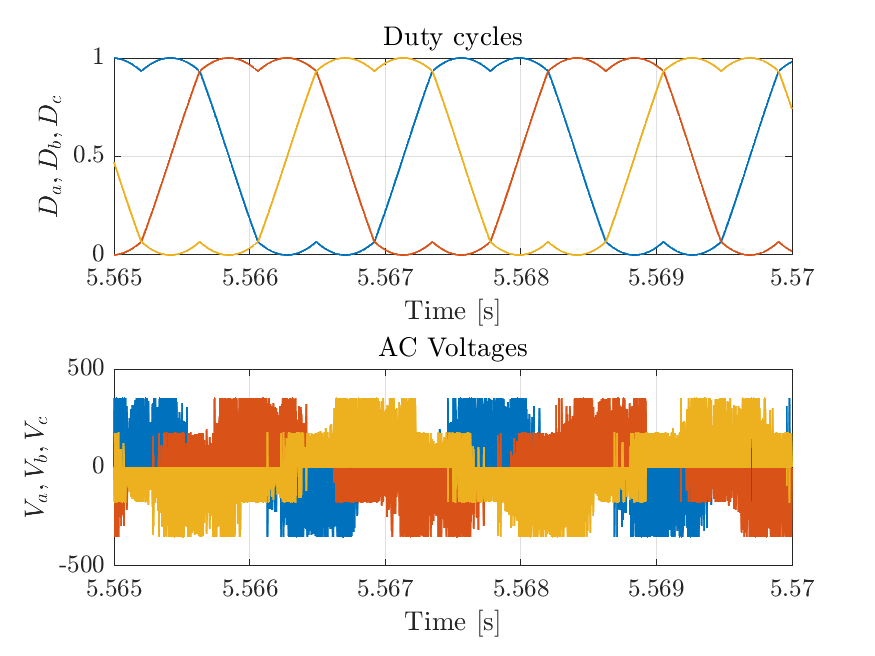
\includegraphics[width=0.85\linewidth]{fig/abc_plot.png}
    \caption{Duty cycles y tensiones alternas.}
    
\end{figure}


Por ello se desarrolla un modelo en PLECS que incorpora el lazo de control, el inversor con MOSFETs, la planta mecánica simplificada, y a la cual se le discretiza la adquisición y el control, de manera que es una aproximación muy realista de la posterior implementación en un microcontrolador.

********CAPTURAS MODELO PLECS********

\begin{figure}[!ht]
    \centering

    \begin{subfigure}{0.4\textwidth}
        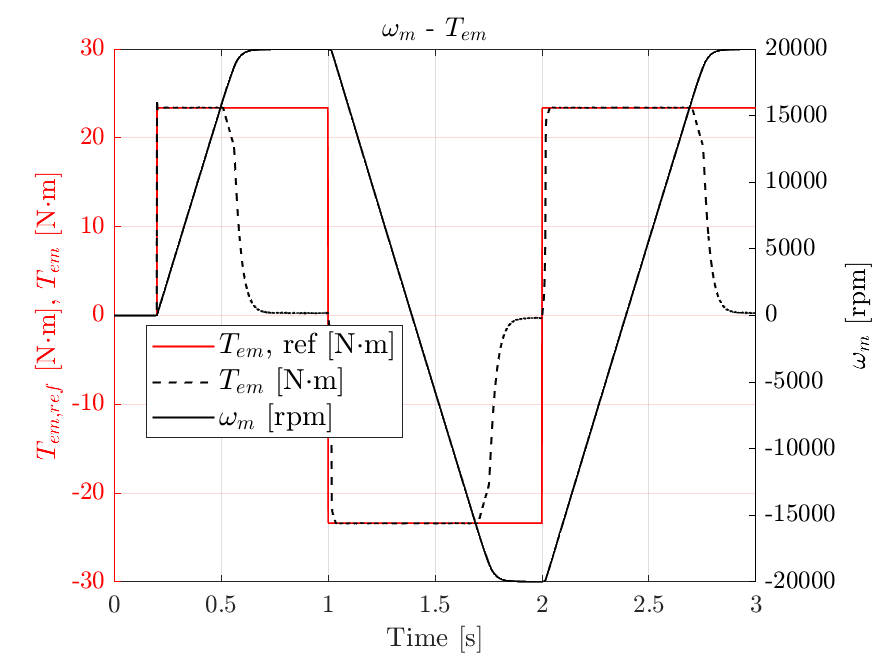
\includegraphics[width=\linewidth]{fig/PLECS_Tem.png}
        \caption{Torque electromagnético ($T_{em}$) vs Velocidad mecánica ($\omega_{m}$)}
    \end{subfigure}
    %
    \begin{subfigure}{0.4\textwidth}
        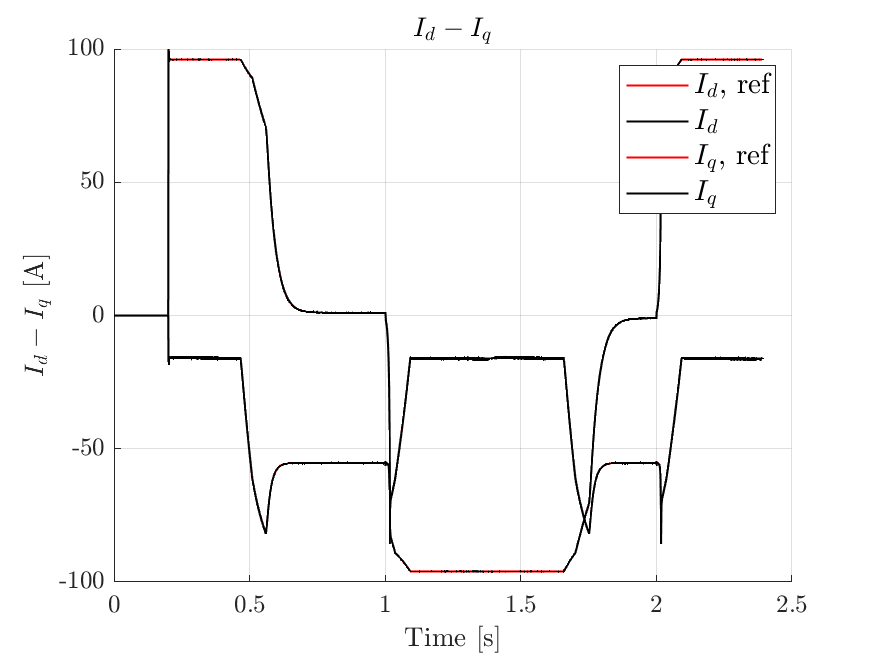
\includegraphics[width=\linewidth]{fig/PLECS_idiq.png}
        \caption{Corrientes ($I_{d} - I_{q}$)}
    \end{subfigure}

    \begin{subfigure}{0.4\textwidth}
        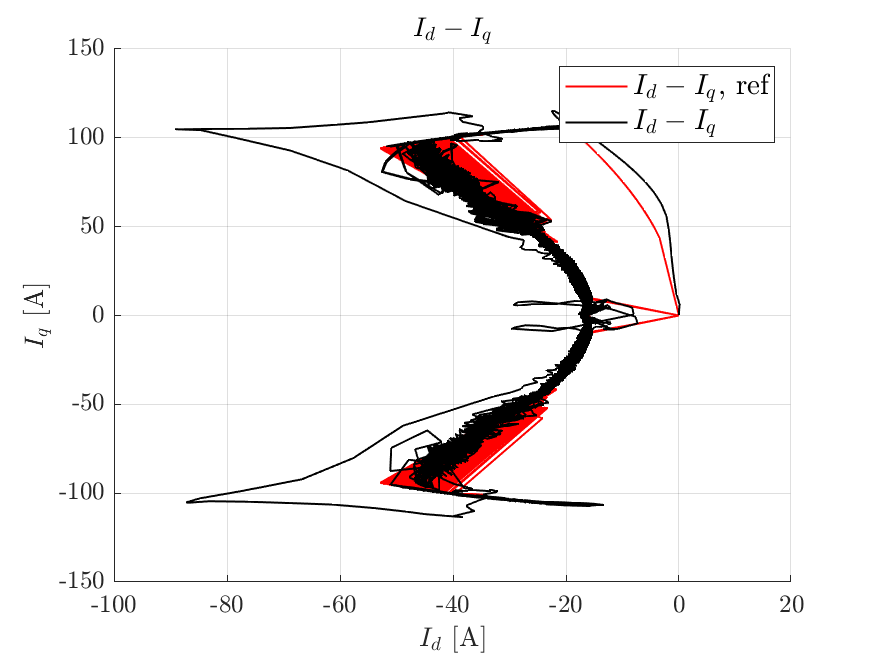
\includegraphics[width=\linewidth]{fig/PLECS_id-iq.png}
        \caption{Corriente ($I_{d}$) vs Corriente ($I_{q}$)}
    \end{subfigure}
    %
    \begin{subfigure}{0.4\textwidth}
        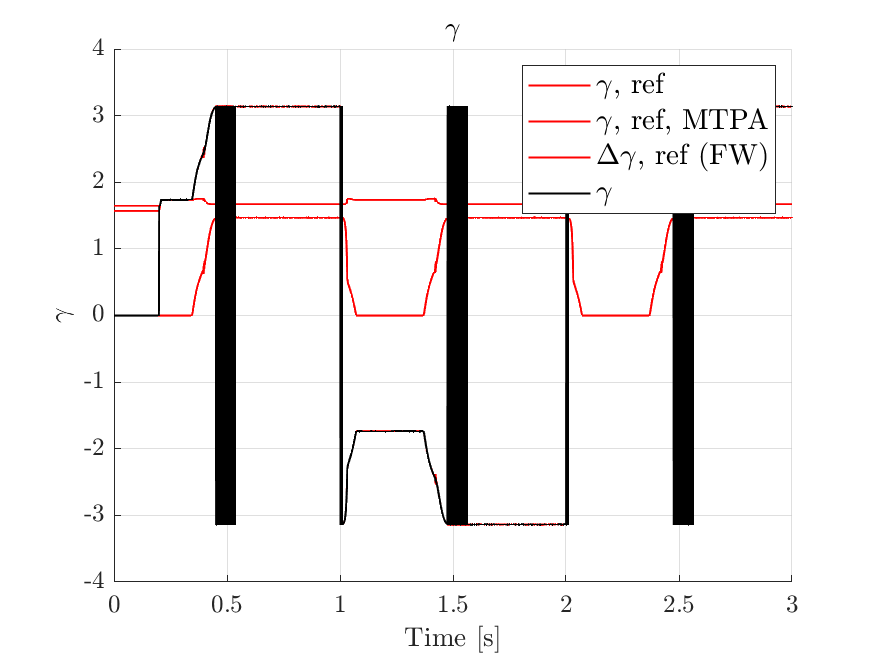
\includegraphics[width=\linewidth]{fig/PLECS_gamma.png}
        \caption{Ángulo de corriente ($\gamma$)}
    \end{subfigure}

    \begin{subfigure}{0.4\textwidth}
        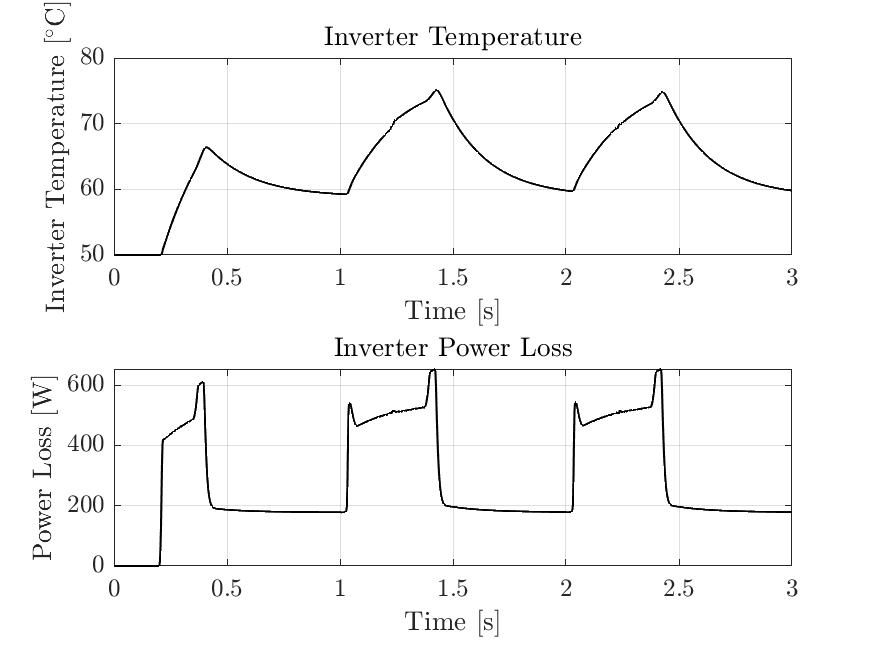
\includegraphics[width=\linewidth]{fig/PLECS_thermal.png}
        \caption{Temperatura y pérdidas del inversor}
    \end{subfigure}
    %
    \begin{subfigure}{0.4\textwidth}
        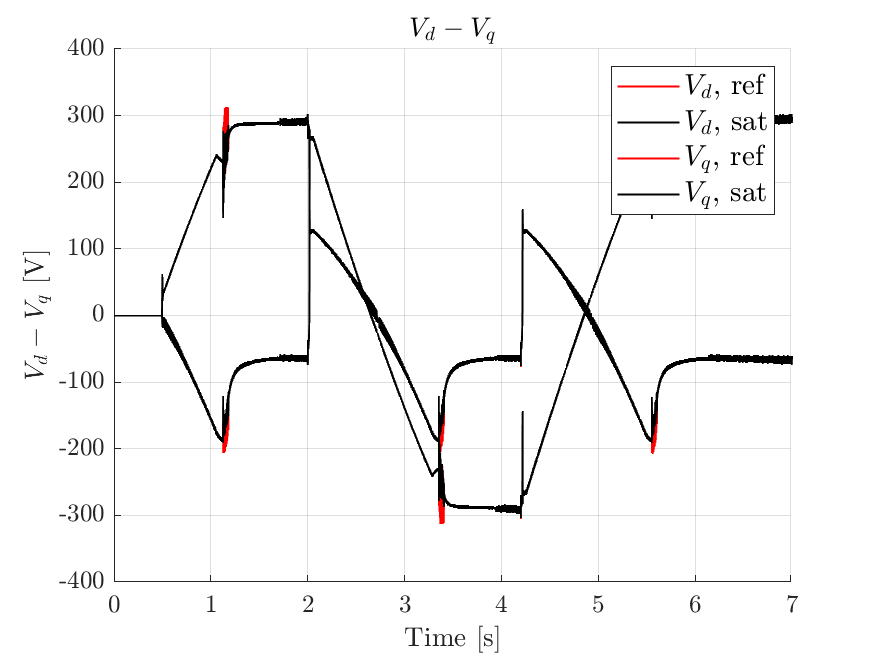
\includegraphics[width=\linewidth]{fig/PLECS_vdvq.png}
        \caption{Voltajes ($V_{d} - V_{q}$)}
    \end{subfigure}

    \caption{Resultados de la simulación.}
\end{figure}



\section{\textit{Hardware}}

\subsection{Requisitos y pre-concepto}

Para definir los requisitos del inversor, se deben considerar las restricciones del tren de potencia que impone la normativa, así como

\subsection{Concepto}
Con el fin de producir las tensiones trifásicas que calcula el control se implementa un ondulador trifásico fuente de voltaje (VSI). Existen varias topologías que permiten hacer un ondulador trifásico, pero la más utilizada es el VSI de 2 niveles, formado por tres ramas de medio puente. Otras topologías de más niveles logran sintetizar tensiones con menos distorsión armónica, pero dado que lo que importa realmente para una controladora de motores eléctricos es la corriente.

\begin{figure}[!ht]

    \centering
    \begin{circuitikz}
        % Upper MOSFETs
        \draw (0,0) node[nigfete,anchor=D,bodydiode] (M1) {};
        \draw (2,0) node[nigfete,anchor=D,bodydiode] (M2) {};
        \draw (4,0) node[nigfete,anchor=D,bodydiode] (M3) {};

        % Lower MOSFETs
        \draw (0,-2) node[nigfete,anchor=D,bodydiode] (M4) {};
        \draw (2,-2) node[nigfete,anchor=D,bodydiode] (M5) {};
        \draw (4,-2) node[nigfete,anchor=D,bodydiode] (M6) {};

        % Connections
        \draw (M1.S) -- (M4.D);
        \draw (M2.S) -- (M5.D);
        \draw (M3.S) -- (M6.D);
        \draw (M1.D) -- (M2.D) -- (M3.D);
        \draw (M4.S) -- (M5.S) -- (M6.S);

        % Battery
        \draw (M1.D)  |-  ++(-4,0) to[battery, l=$V_{\text{DC}}$] ++(0,-3.5)  |-  (M4.S);
        \draw (M1.D)  |-  ++(-1.5,0) to[capacitor] ++(0,-3.5)  |-  (M4.S);

        % Phase cables
        \draw (M3.S)  |-  ++(2,-0.5) node[right, font=\tiny] {C};
        \draw (M2.S)  |-  ++(4,-0.25) node[right, font=\tiny] {B};
        \draw (M1.S)  |-  ++(6,0) node[right, font=\tiny] {A};

    \end{circuitikz}
        \caption{VSI con MOSFETs.}

\end{figure}

Ya que el convertidor implementa código propio, se decide implementar dos VSI en el mismo convertidor, de modo que se opta por unificar algunos elementos de ambos como la refrigeración con el fin de optimizar el peso y el espacio. Esta decisión evita duplicados de medidas, componentes y software, sin embargo, lleva a ciertas complicaciones de ensamblaje. Además, el microcontrolador deberá ser capaz de ejecutar los dos lazos de control en el mismo tiempo.

Con tal de adquirir las variables necesarias para el control y interfazar con el coche y periféricos, son necesarios los ******* que se muestran en este diagrama de bloques.

********DIAGRAMA DE BLOQUES********

El convertidor se divide en 3 PCBs, que se listan a continuación:

\begin{itemize}
	\item Inverter Power
	\item Inverter DC
	\item Inverter Control
\end{itemize}

Como su nombre indica, \textit{Inverter Power} alojará todos los componentes de potencia, incluyendo los \textit{gate drivers}, los sensores de corriente, los semiconductores, los buses de continua y los conectores de potencia. Esta PCB se fabrica en duplicado ya que contiene todos los elementos que son necesarios repetir para el control de dos motores.

En \textit{Inverter DC} se puede encontrar el sensado de la tensión de los buses, el circuito de descarga, y la detección de alta tensión para la \textit{TSAL}.

Por su parte, \textit{Inverter Control} contiene el microcontrolador de la familia STM32F7 para accionar los \textit{gate drivers}, así como para realizar las lecturas de corriente, tensión y temperatura, las interfaces con los sensores de posición de los motores o los protocolos comunicación.

El montaje de estas placas se realiza de forma compacta y eficiente, de manera que quepa una placa refrigerada entre medias para controlar la temperatura de los semiconductores de ambos inversores. Se encajan de manera que la placa de control se puede conectar a las placas de potencia mediante conectores \textit{board-to-board}, y la PCB del bus de continua se sitúa estratégicamente cerca del conector de la batería. Las conexiones de potencia facilitan la integración con el cableado del monoplaza debido a su posicionamiento.


\subsection{Semiconductores}

\subsubsection{Elección del Material: Carburo de Silicio (SiC)}

La decisión de emplear carburo de silicio (SiC) como material para los semiconductores se fundamenta en consideraciones específicas de la aplicación y en los requisitos críticos de la competición. En un entorno donde la reducción de peso y volumen es crucial, el SiC emerge como una opción destacada, especialmente dado que el precio no es una restricción principal en este contexto, dado que el atractivo del proyecto ha logrado captar la atención de empresas que han proporcionado muestras para el desarrollo del convertidor.

Las ventajas inherentes del SiC, como su rendimiento superior o su resistencia a temperaturas más altas, permiten un diseño más compacto y robusto del inversor de tracción. Estas características son esenciales para cumplir con los rigurosos requisitos de un monoplaza de competición, donde la optimización del peso y del espacio es fundamental para lograr altas densidades de potencia.

\subsubsection{Módulos de Potencia: Selección y Comparativa}

En el diseño del inversor de tracción, se optó por módulos \textit{half-bridge} debido a su idoneidad para el rango de potencias y tensiones del convertidor. Dos modelos de semiconductores se consideraron para su integración: el DFS05HF12EYR1 de Leapers Semiconductor y el CAB016M12FM3 de Wolfspeed.

Ambos modelos cumplen estrictamente con los requisitos de la aplicación, con un voltaje de ruptura (\(V_{DS,breakdown}\)) superior a 1200V y una corriente máxima (\(I_{DS,max}\)) que excede los 80 ARMS. La elección de dos modelos distintos se basa en la intención de realizar pruebas comparativas para verificar las diferencias entre ambos.

El DFS05HF12EYR1 ofrece especificaciones muy buenas en su datasheet, aunque Leapers Semiconductors no lleva muchos años en la industria y no han logrado crear la confianza que otras empresas han conseguido con su experiencia. Por otro lado, el CAB016M12FM3, de la reconocida marca Wolfspeed, aporta la confiabilidad asociada a una empresa con amplia experiencia en el campo.

Según sus respectivos datasheets, ambos modelos permiten alcanzar sin mucho esfuerzo una frecuencia de conmutación de 50 kHz, lo que contribuye significativamente a la reducción del tamaño del bus de continua y optimiza el empaquetado del inversor. La placa de potencia se diseñará para permitir la prueba de ambos modelos, ya que comparten \textit{footprint}, facilitando la adaptabilidad y la evaluación comparativa.

\subsubsection{Análisis de Pérdidas}

El análisis de pérdidas en los semiconductores se ha llevado a cabo mediante simulaciones detalladas utilizando herramientas especializadas. Estas simulaciones se centran en evaluar las pérdidas de conducción y conmutación de los MOSFETs y diodos por separado, permitiendo una comprensión profunda de su comportamiento en diversas condiciones de operación.

Para los semiconductores de Wolfspeed, las simulaciones fueron validadas mediante herramientas proporcionadas por el fabricante, añadiendo una capa adicional de confiabilidad a los resultados obtenidos. La metodología de simulación asume la entrega continua de la potencia máxima, permitiendo el diseño de la coldplate basándose en la determinación del porcentaje de la potencia máxima equivalente en un perfil de conducción realista.

Las herramientas utilizadas para la evaluación de pérdidas incluyen PLECS para simulaciones de sistema y LTSPICE para ensayos \textit{double pulse}.

\subsubsection{Sistema de Refrigeración}

Como es de esperar, la elección del sistema de refrigeración para los semiconductores se ha dirigido hacia una coldplate de agua. Esta elección se fundamenta en la necesidad de mantener una interfaz de temperatura fija para los semiconductores, lo que simplifica el diseño del sistema. La experiencia previa del equipo en sistemas de refrigeración por agua también influyó en esta decisión, proporcionando un marco confiable para la implementación.

A pesar de que los semiconductores de carburo de silicio (SiC) tienen una temperatura máxima de unión (\(T_{j(max)}\)) notablemente alta, se establece como objetivo mantener el delta de temperatura (\(\Delta T\)) por debajo de 30 ºC. Este enfoque busca garantizar una operación óptima y una vida útil prolongada de los componentes, además de mitigar los posibles efectos negativos derivados del calor.

\subsection{\textit{Gate drivers}}

Calculo y seleccion de los GD

\subsection{Bus de condensadores}

Justificacion de su existencia

cálculo de Irms y Vrip

Selección

\subsection{Conductores}

Pletinas

Cables

Conectores

Análisis de parasitos (Lcable), etc.

\subsection{PCB de potencia}

explicacion del concepto y de la(s) PCB

justificacion de conectores / interfaces

justificacion numero de capas, etc.

\subsection{PCB de control}

explicacion del concepto y de la(s) PCB

justificacion de conectores / interfaces

justificacion numero de capas, etc.

\subsection{PCB de TS-DC}

explicacion del concepto y de la(s) PCB

justificacion de conectores / interfaces

justificacion numero de capas, etc.

\section{\textit{Software}}

\subsection{Concepto}

Diagrama de bloques de software, justificado (ojo, detallar el dual)

Abstraccion ECU, estandarizacion, RTOS

Shield con seleccion de microcontrolador


\subsection{Retos}

velocidad MCU

sincronizacion de ambos inversores

mensajes con el coche

\subsection{Tareas}

Init

ADCs

Comunicaciones

PWMs

Flash o EEPROM

Seguridad

\subsection{Interfaz de usuario}

justificar ausencia de UI integrada

Interfaz de HW 

PlotJuggler

Debugger

Actualizacion de parametros por CAN

\section{Validación}
xd

